\documentclass[thesis.tex]{subfiles}
\usepackage{xr} 
\externaldocument[Pi:]{aux/periodic}

\begin{document}

% remove this eventually or do conditional
\chapter{KdV5 with periodic boundary conditions}

\section{Proof of Existence Theorems}

\subsection{Proof of Initial Lemmas}

\newtheorem*{lemma:psiform}{Lemma \ref{Pi:psiform}}
\begin{lemma:psiform}
Let $H$ be the Hamiltonian from Hypothesis \ref{Pi:Hhyp}. Then $\Psi(x) = \nabla H(Q(x))$.
\begin{proof}
Since \eqref{Pi:genODE} is Hamiltonian, $\langle F(Q(x)), \nabla H(Q(x)) \rangle = 0$ for all $x$. Taking the gradient of this and using known vector calculus identities,
\begin{align*}
0 &= \nabla \langle F(Q(x)), \nabla H(Q(x)) \rangle \\
&= D F(Q(x))^* \nabla H(Q(x)) + D^2 H(Q(x))^* F(Q(x)) \\
&= D F(Q(x))^* \nabla H(Q(x)) + D^2 H(Q(x)) Q'(x) \\
&= D F(Q(x))^* \nabla H(Q(x)) + \frac{d}{dx} \nabla H(Q(x))
\end{align*}
since the Hessian matrix is self-adjoint. Rearranging this,
\begin{equation*}
\frac{d}{dx} \nabla H(Q(x)) = -D F(Q(x))^* \nabla H(Q(x)) 
\end{equation*}
thus $\nabla H(Q(x))$ is a solution to the adjoint variational equation \eqref{Pi:adjvareq1}. Since $\nabla H$ is continuous and $Q(x)$ is bounded (it decays exponentially to 0 at $\pm \infty$), $\nabla H(Q(x))$ is bounded as well. By Hypothesis \ref{Pi:nondegenhyp}, there is a unique such solution. It follows that $\Psi(x) = \nabla H(Q(x))$.
\end{proof}
\end{lemma:psiform}

\newtheorem*{lemma:eigadjoint}{Lemma \ref{Pi:eigadjoint}}
\begin{lemma:eigadjoint}
Consider the linear ODE $V' = A(x)V$ and the corresponding adjoint equation $W' = -A(x)^* W$, where $A$ is an $n \times n$ matrix depending on $x$. Then the following are true.
\begin{enumerate}[(i)]
\item $\dfrac{d}{dx}\langle V(x), W(x) \rangle = 0$, thus the inner product is constant in $x$.
\item If $\Phi(y, x)$ is the evolution operator for $V' = A(x)V$, then $\Phi(x, y)^*$ is the evolution operator for the adjoint problem $W' = -W(x)^* W$.
\end{enumerate}
\begin{proof}
For (i), take the derivative of the inner product and use the expressions for $V'$ and $W'$. For (ii), take the derivative of the expression $\Phi(y, x)\Phi(x, y) = I$.
\end{proof}
\end{lemma:eigadjoint}

\subsection{Exponential Dichotomy}

Let $\Phi_\pm(x, y; \beta^\pm)$ be the family of evolution operators for the ODEs
\begin{align}\label{qpmODEs}
(V^\pm)' &= D F(Q^\pm(x, \beta^\pm)(x)) V^\pm && x \in \R^\pm
\end{align}
In the next lemma, we decompose these evolution operators via exponential dichotomies on $\R^+$ and $\R^-$.

% lemma : exp dichotomy

\begin{lemma}\label{dichotomy1}
There exist projections
\begin{align*}
&P_+^s(y; \beta^+) && y \geq 0 \\
&P_+^u(y; \beta^+) = I - P_+^s(y; \beta^+) && y \geq 0 \\
&P_-^u(y; \beta^-) && y \leq 0 \\
&P_-^s(y; \beta^-) = I - P_-^u(y; \beta^-) && y \leq 0 \\
\end{align*}
such that the evolution operators $\Phi_\pm(x, y; \beta^\pm)$ can be decomposed as
\begin{align*}
\Phi^s_\pm(x, y; \beta^\pm) &= \Phi_\pm(x, y; \beta^\pm) P^s_\pm(y; \beta^\pm) \\
\Phi^u_\pm(x, y; \beta^\pm) &= \Phi_\pm(x, y; \beta^\pm) P^u_\pm(y; \beta^\pm) 
\end{align*}
where we have the estimates
\begin{align*}
|\Phi^s_+(x, y, \beta^+)| &\leq C e^{-\alpha(x - y)} && 0 \leq y \leq x \\
|\Phi^u_+(x, y, \beta^+)| &\leq C e^{-\alpha(y - x)} && 0 \leq x \leq y \\
|\Phi^u_-(x, y, \beta^-)| &\leq C e^{-\alpha(y - x)} && 0 \geq y \geq x \\
|\Phi^s_-(x, y, \beta^-)| &\leq C e^{-\alpha(x - y)} && 0 \geq x \geq y \\
\end{align*}
which also hold for derivatives with respect to the initial conditions $\beta^\pm$. In addition, the projections satisfy the commuting relations
\begin{align*}
\Phi_\pm(x, y; \beta^\pm) P^{s/u}_\pm(y; \beta^\pm) 
= P^{s/u}_\pm(x; \beta^\pm) \Phi_\pm(x, y; \beta^\pm)
\end{align*}
Finally, the projections can be chosen such that at $y = 0$ we have, independent of $\beta^+$ and $\beta^-$
\begin{align*}
\ker P^s_+(0; \beta^+) &= Z \oplus Y^- \\
\ker P^u_-(0; \beta^-) &= Z \oplus Y^+ \\
\ran P^u_+(0; \beta^+) &= Z \oplus Y^- \\
\ran P^s_-(0; \beta^-) &= Z \oplus Y^+
\end{align*}

\begin{proof}
Since $DF(0)$ is hyperbolic by Hypothesis \ref{Pi:hypeqhyp}, this follows from Lemma 5.1 in \cite{Sandstede1997}, which follows from Lemma 1.1 in \cite{Sandstede1993}.
\end{proof}
\end{lemma}

The next lemma provides a bound on the difference between the exponential dichotomy projections and the projections onto the stable and unstable eigenspaces of $DF(0)$.

% lemma : bound on projection difference

\begin{lemma}\label{projdifflemma}
We have the following estimates
\begin{equation}\label{projdiffest}
\begin{aligned}
|P^u_+(x; \beta^+) - P_0^u| &\leq C e^{-\alpha x} \\
|P^s_+(x; \beta^+) - P_0^s| &\leq C e^{-\alpha x} \\
|P^u_-(x; \beta^-) - P_0^u| &\leq C e^{\alpha x} \\
|P^s_-(x; \beta^-) - P_0^s| &\leq C e^{\alpha x} 
\end{aligned}
\end{equation}
where $P_0^s$ and $P_0^u$ are the projections onto the stable and unstable eigenspaces $E_0^s$ and $E_0^u$ of $DF(0)$. The estimates are independent of $\beta_i^\pm$.
\begin{proof}
This follows from Lemma 1.1 and Lemma 2.1 in San93.
\end{proof}
\end{lemma}

\subsection{Fixed Point Formulation}

In this section, we formulate equation \eqref{Pi:exsystem1} as a fixed point problem. First, we plug in the piecewise ansatz \eqref{Pi:Upiecewise}into \eqref{Pi:genODE}. Thus, for $i = 0, \dots, n-1$, 
\begin{align*}
U_i^\pm(x)' &= (Q^\pm(x; \beta_i^\pm))' + V_i^\pm(x)' = F\left(Q^\pm(x; \beta_i^\pm) + V_i^\pm(x) \right) \\
\end{align*}
Since $Q^\pm(x; \beta_i^\pm)$ solves \eqref{Pi:genODE} on $\R^\pm$, 
\begin{align*}
(V_i^\pm(x))' &= F\left(Q^\pm(x; \beta_i^\pm) + V_i^\pm(x) \right) - F(Q^\pm(x; \beta_i^\pm))
\end{align*}
Expanding the RHS in a Taylor series (using the version for Banach spaces) about $Q^\pm(x; \beta_i^\pm)$, we attain the ODE for $V_i^\pm$.
\begin{equation}\label{Vpiecewise}
(V_i^\pm(x))' = DF(Q^\pm(x; \beta_i^\pm)) V_i^\pm(x) + G_i^\pm(x; \beta_i^\pm, V_i^\pm)
\end{equation}
where 
\begin{equation}\label{Gquadratic}
G_i^\pm(\beta_i^\pm, V_i^\pm)(x) = \mathcal{O}(|V_i^\pm|^2)
\end{equation}
This estimate is independent of the parameters $\beta_i^\pm$ since we can get a uniform bound for $Q^\pm(0, \beta_i^\pm)$ for sufficiently small $\beta_i^\pm$. As in \cite{Sandstede1997}, derivatives of $G_i^\pm$ with respect to the parameters $\beta_i^\pm$ are the same order in $V_i^\pm$.

We now rewrite the piecewise differential equations \eqref{Vpiecewise} in integrated form to attain the fixed point equations.
\begin{equation}\label{FPequations}
\begin{aligned}
V_i^+(x) &= \Phi^u_+(x, X_i; \beta_i^+) a_i^+  \\
&+ \int_{X_i}^x \Phi_+^u(x, y; \beta_i^+) G_i^+(y; V_i^+(y),\beta_i^+)dy \\
&+ \int_0^x \Phi_+^s(x, y; \beta_i^+) G_i^+(y; V_i^+(y),\beta_i^+)dy \\ 
V_i^-(x) &= \Phi^s_-(x, -X_{i-1}; \beta_i^-) a_{i-1}^-  \\
&+ \int_{-X_{i-1}}^x \Phi_-^s(x, y; \beta_i^-) G_i^-(y; V_i^-(y),\beta_i^-)dy \\
&+ \int_0^x \Phi_-^u(x, y; \beta_i^-) G_i^-(y; V_i^-(y),\beta_i^-)dy \\
\end{aligned}
\end{equation}
where for the initial conditions $a_i^\pm$ at $-X_{i-1}$ and $X_i^+$, we take $a_i^+ \in E_0^u$ and $a_i^- \in E_0^s$. We do not have initial conditions at $x = 0$ for the other side of the dichotomy since those initial conditions are incorporated into $\beta_i^\pm$.

Finally, define the exponentially weighted norms
\begin{equation}\label{expwtnorm}
\begin{aligned}
||V||_{X, +} &= \sup_{x \in [0, X]} e^{\alpha(X - x)}|V(x)| \\
||V||_{X, -} &= \sup_{x \in [-X, 0]} e^{\alpha(X + x)}|V(x)|
\end{aligned}
\end{equation}
Let $K_{X, \pm}$ be the spaces of continuous functions on $[0, X]$ and $[-X, 0]$ equipped with these norms. These are known to be Banach spaces. Let $B_{X, \pm}(\rho)$ be the ball of radius $\rho$ about $0$ in these spaces.

\subsection{Inversion}

We will solve for the functions $V_i^\pm$ and initial conditions $\beta_i^\pm$ in a series of lemmas. First, we will solve for the functions $V_i^\pm(x)$ in terms of the initial conditions $a_i^\pm$. Note that $V_i^+(x)$ only depends on $a_i^+$ and $V_i^-(x)$ only depends on $a_{i-1}^-$.

% lemma : solve for V_i^\pm

\begin{lemma}\label{solveforV}
There exist $\delta, \rho > 0$ such that for $|X_i|, |X_{i-1}| > 1/\delta$ and $|a_{i-1}^-|, |a_i^+|, |\beta_i^\pm| < \delta$, there exist unique solutions
\begin{align*}
V_i^-(a_{i-1}^-, \beta_i^-) &\in B_{X_{i-1}, -}(\rho) \\
V_i^+(a_i^+, \beta_i^+) &\in B_{X_i, +}(\rho) \\
\end{align*}
to the fixed point equations \eqref{FPequations}. $V_i^-(a_{i-1}, \beta_i^-)$ depends smoothly on $(a_{i-1}^-, \beta_i^-)$, and $V_i^+(a_i, \beta_i^+)$ depends smoothly on $(a_i^+, \beta_i^+)$. Finally, we have the estimates
\begin{equation}\label{Vest}
\begin{aligned}
||V_i^-||_{X_{i-1}, -} &\leq C |a_{i-1}^-| \\
||V_i^+||_{X_i, +} &\leq C |a_i^+|
\end{aligned}
\end{equation}
where the constant $C$ depends only on $\delta$. These estimates hold as well for derivatives of $V_i^\pm$ with respect to $\beta_i^\pm$.
\begin{proof}
The proof follows that of Lemma 5.2 in \cite{Sandstede1997}. Since we can deal with each of the $2n$ pieces separately, we will do only the pieces on $\R^+$ here; the pieces on $\R^-$ are similar.

The RHS of the fixed point equation \eqref{FPequations} on $\R^+$ defines a smooth mapping on $K_{X_i, +}$. We need to verify that the RHS maps $K_{X_i, +} \mapsto K_{X_i, +}$. To do this, we obtains bounds on three terms on the RHS individually using the estimates on $\Phi^{s/u}_\pm$ from Lemma \ref{dichotomy1}. For the first term on the RHS,
\begin{align*}
e^{\alpha(X_i - x)} | \Phi^u_+(x, X_i; \beta_i^+) a_i^+ | 
&\leq C e^{\alpha(X_i - x)} e^{-\alpha(X_i - x)} |a_i^+| \\
&\leq C |a_i^+|
\end{align*}
For the second term, we also use the estimate on $G$ from \eqref{Gquadratic}, and the fact that $V_i^+ \in K_{X_i, +}$. 
\begin{align*}
e^{\alpha(X_i - x)} &\left| \int_{X_i}^x \Phi_+^u(x, y; \beta_i^+) G_i^+(y, V_i^+(y),\beta_i^+)dy  \right| \\
&\leq C e^{\alpha(X_i - x)} \int_x^{X_i} e^{-\alpha(y - x)}|V_i^+(y)|^2 dy \\
&\leq C e^{\alpha(X_i - x)} \int_x^{X_i} 
e^{-\alpha(y - x)}(e^{-\alpha(X_i - y)})^2|e^{\alpha(X_i - y)} V_i^+(y)|^2 dy \\
&\leq C e^{\alpha(X_i - x)} \int_x^{X_i} 
e^{-\alpha(y - x)}(e^{-\alpha(X_i - y)})^2 dy \\
&\leq C \int_0^{X_i} e^{-\alpha (X_i - y)} dy \\
&\leq C
\end{align*}
The third term is similar. Thus the RHS of the fixed point equation \eqref{FPequations} on $\R^+$ is a smooth map $K_{X_i, +} \mapsto K_{X_i, +}$. 

Define $H: K_{X_i, +} \times E_0^s \rightarrow K_{X_i, +}$ by
\begin{align*}
H(V_i^+(x), a_i^+, \beta_i^+) &= V_i^+(x) - \Phi^u_+(x, X_i; \beta_i^+) a_i^+  \\
&- \int_{X_i}^x \Phi_+^u(x, y; \beta_i^+) G_i^+(y, V_i^+(y),\beta_i^+)dy \\
&- \int_0^x \Phi_+^s(x, y; \beta_i^+) G_i^+(y, V_i^+(y),\beta_i^+)dy 
\end{align*}
which is just the RHS of the fixed point equation \eqref{FPequations} on $\R^+$. Since $Q(x)$ satisfies \eqref{Pi:genODE}, $H(0, 0, 0) = 0$. Since $G$ is quadratic in $V_i^+(x)$, the Fr\'echet derivative of $H$ with respect to $V_i^+(x)$ at $(V_i^+(x), a_i^+, \beta_i^+) = (0, 0, 0)$ is the identity, thus is a Banach space isomorphism on $K_{X_i, +}$. Using the implicit function theorem, we can solve for $V_i^+(x)$ in terms of $(a_i^+, \beta_i^+)$ for sufficiently small $|a_i^+|, |\beta_i^+|$. Since the map $H$ is smooth, this dependence is smooth.

The estimate on $V_i^\pm$ comes from the estimate of the first term on the RHS of the fixed point equations, since the other terms (those involving the integrals) are quadratic in $V_i^\pm(x)$. Since the estimate \eqref{Gquadratic} on $G$ is independent of $\beta_i^\pm$, the estimate on {}$V_i^\pm$ is also independent of $\beta_i^\pm$. Since the exponential dichotomy estimates from Lemma \ref{dichotomy1} hold for derivatives with respect $\beta_i^\pm$, these estimates also hold for derivatives with respect $\beta_i^\pm$.
\end{proof}
\end{lemma}

Using the previous lemma, we have solved equation \eqref{Pi:exsystem1} in our system. Next, we satisfy equation \eqref{Pi:exsystem2}, i.e. $U_i^+(X_i) - U_{i+1}^-(-X_i) = 0$, to match the pieces \eqref{Pi:Upiecewise} at the endpoints $\pm X_i$. This will solve for the initial conditions $a_i^\pm$.

% Lemma : solve for a_i^\pm

\begin{lemma}\label{solvefora}
For any $X_i$ and $\beta_i^\pm$ chosen as in Lemma \ref{solveforV}, there is a unique pair of initial conditions $(a_i^+, a_i^-) \in E_0^s \times E_0^u$ such that $U_i^+(X_i) - U_{i+1}^-(-X_i) = 0$. $(a_i^+, a_i^-)$ depends smoothly on $(\beta_i^+, \beta_{i+1}^-)$, and we have the following estimate, which is independent of $(\beta_i^+, \beta_{i+1}^-)$.
\begin{equation}\label{aest}
|a_i^\pm| \leq C e^{-\alpha X_i}
\end{equation}
This holds as well for derivatives with respect to $\beta_i^\pm$. We also have the following expressions for $a_i^\pm$.
\begin{equation}\label{aiformula}
\begin{aligned}
a_i^+ &= -P^u_0 \left( Q^+(X_i; \beta_i^+) - Q^-(-X_i; \beta_{i+1}^-) \right) + \mathcal{O}( e^{-2 \alpha X_i} ) \\
a_i^- &= P^s_0 \left( Q^+(X_i; \beta_i^+) - Q^-(-X_i; \beta_{i+1}^-) \right) + \mathcal{O}\left( e^{-2 \alpha X_i} \right)
\end{aligned}
\end{equation}

\begin{proof}
First, we plug in the fixed point equations \eqref{FPequations} to the expressions \eqref{Pi:Upiecewise} for $U_i^+$ and $U_{i+1}^-$ and evaluate them at $\pm X_i$ to get
\begin{align*}
U_i^+(X_i) &= Q^+(X_i; \beta_i^+) + P^u_+(X_i; \beta_i^+) a_i^+ \\
&+ \int_0^{X_i} \Phi_+^s(X_i, y; \beta_i^+) G_i^+(y, V_i^+(y),\beta_i^+)dy \\ 
U_{i+1}^-(-X_i) &= Q^-(-X_i; \beta_{i+1}^-) + P^s_-(-X_i; \beta_{i+1}^-) a_i^- \\
&+ \int_0^{-X_i} \Phi_-^u(-X_i, y; \beta_{i+1}^-) G_{i+1}^-(y, V_{i+1}^-(y),\beta_{i+1}^-)dy \\
\end{align*}
Adding and subtracting the projections $P_0^s$ and $P_0^u$ and recalling that $a_i^+ \in \in E_0^u$ and $a_i^- \in E_0^s$, this becomes
\begin{align*}
U_i^+(X_i) &= Q^+(X_i; \beta_i^+) + a_i^+ + (P^u_+(X_i; \beta_i^+) -  P^u_0)a_i^+ \\
&+ \int_0^{X_i} \Phi_+^s(X_i, y; \beta_i^+) G_i^+(y, V_i^+(y),\beta_i^+)dy \\ 
U_{i+1}^-(-X_i) &= Q^-(-X_i; \beta_{i+1}^-) + a_i^- + (P^s_-(-X_i; \beta_{i+1}^-) - P^s_0) a_i^- \\ 
&+ \int_0^{-X_i} \Phi_-^u(-X_i, y; \beta_{i+1}^-) G_{i+1}^-(y, V_{i+1}^-(y),\beta_{i+1}^-)dy
\end{align*}
Subtract these to get $H: E_0^s \times E_0^u \times \R \times \R \rightarrow \R^{2m}$, defined by
\begin{align*}
H(a_i^+, &a_i^-, \beta_i^+, \beta_{i+1}^-) 
= a_i^+ - a_i^- + (P^u_+(X_i; \beta_i^+) -  P^u_0)a_i^+ - (P^s_-(-X_i; \beta_{i+1}^-) - P^s_0) a_i^-  \\
&+ Q^+(X_i; \beta_i^+) - Q^-(-X_i; \beta_{i+1}^-)\\
&+ \int_0^{X_i} \Phi_+^s(X_i, y; \beta_i^+) G_i^+(y, V_i^+(y),\beta_i^+)dy
- \int_0^{-X_i} \Phi_-^u(-X_i, y; \beta_{i+1}^-) G_{i+1}^-(y, V_{i+1}^-(y),\beta_{i+1}^-)dy 
\end{align*}
We need to solve $H(a_i^+, a_i^-, \beta_i^+, \beta_{i+1}^-) = 0$ for $a_i^\pm$. Plugging in the solution for $V_i^\pm(x)$ from Lemma \ref{solveforV}, this becomes
\begin{align*}
H(a_i^+, &a_i^-, \beta_i^+, \beta_{i+1}^-) \\
&= a_i^+ - a_i^- + (P^u_+(X_i; \beta_i^+) -  P^u_0)a_i^+ - (P^s_-(-X_i; \beta_{i+1}^-) - P^s_0) a_i^-  \\
&+ Q^+(X_i; \beta_i^+) - Q^-(-X_i; \beta_{i+1}^-) \\
&+ \int_0^{X_i} \Phi_+^s(X_i, y; \beta_i^+) G_i^+(y, V_i^+(a_i^+, \beta_i^+)(y),\beta_i^+)dy \\
&- \int_0^{-X_i} \Phi_-^u(-X_i, y; \beta_{i+1}^-) G_{i+1}^-(y, V_{i+1}^-(a_i^-, \beta_{i+1}^-)(y),\beta_{i+1}^-)dy 
\end{align*}

Again, since $Q(x)$ satisfies \eqref{Pi:genODE}, $H(0, 0, 0, 0) = 0$. To  solve for $a_i^\pm$ using the implicit function theorem, we need to evaluate $D_{a_i^\pm} H(0, 0, 0, 0)$. When we take the partial derivatives with respect to $a_i^\pm$ at $a_i^\pm = 0$, the derivatives of the integral terms will be 0 since $G_i^\pm$ is quadratic order in $V_i^\pm$, thus quadratic order in $a_i^\pm$ by Lemma \ref{solveforV}. The $Q^\pm$ terms do not involve $a_i^\pm$. Using the estimate \eqref{projdiffest} from Lemma \ref{projdifflemma}, we have 
\[
\frac{\partial}{\partial a_i^\pm} H(0, 0, 0, 0) = \pm 1 + \mathcal{O} (e^{-\alpha X_i})
\]
For sufficiently large $X_i$, $D_{a_i^\pm} H(0, 0, 0, 0)$ is invertible in a neighborhood of $(0, 0, 0, 0)$. Thus we can use the IFT to solve for $a_i^\pm$ in terms of $\beta_i^\pm$. 

To obtain an expression and estimates for the $a_i^\pm$, we apply the projections $P^u_0$ and $P^s_0$ in turn to $H(a_i^+, a_i^-, \beta_i^+, \beta_{i+1}^-) = 0$. Using $P^u_0$, we have
\begin{equation}\label{Ps0aiplus}
\begin{aligned}
0 &= a_i^+ + P^u_0(P^u_+(X_i; \beta_i^+) -  P^u_0)a_i^+ 
+ P^u_0 \left( Q^+(X_i; \beta_i^+) - Q^-(-X_i; \beta_{i+1}^-) \right)\\
&+ P^u_0 \left( \int_0^{X_i} \Phi_+^s(X_i, y; \beta_i^+) G_i^+(y, V_i^+(a_i^+, \beta_i^+)(y),\beta_i^+)dy \right) \\
&- P^u_0 \left( \int_0^{-X_i} \Phi_-^u(-X_i, y; \beta_{i+1}^-) G_{i+1}^-(y, V_{i+1}^-(a_i^-, \beta_{i+1}^-)(y),\beta_{i+1}^-) dy \right)
\end{aligned}
\end{equation}
We can get estimates for all of these terms. For the first term, we use the estimate \eqref{projdiffest} from Lemma \ref{projdifflemma} to get 
\begin{align*}
|P^u_0(P^u_+(X_i; \beta_i^+) -  P^u_0)a_i^+ | &\leq C e^{-\alpha X_i} |a_i^+|
\end{align*}
For the second term, we use the decay rates of $Q^\pm$ to get
\begin{align*}
|P^u_0 \left( Q^+(X_i; \beta_i^+) - Q^-(-X_i; \beta_{i+1}^-)  \right)| &\leq C e^{-\alpha X_i}
\end{align*}
For the integral terms, we use Lemma \ref{solveforV} to get
\begin{align*}
\left| \int_0^{X_i} \Phi_+^s(X_i, y; \beta_i^+) G_i^+(y, V_i^+(a_i^+, \beta_i^+)(y),\beta_i^+)dy \right| &\leq C \int_0^{X_i}e^{-\alpha(X_i - y)} |V_i^+(y)|^2 dy \\
&\leq C \int_0^{X_i}e^{-3 \alpha (X_i - y)} |e^{\alpha(X_i - y)} V_i^+(y)|^2 dy \\
&\leq C \int_0^{X_i}e^{-3 \alpha (X_i - y)} (||V_i^+||_{X_i, +})^2 dy \\
&\leq C |a_i^+|^2
\end{align*}
The other integral term is similar. Substituting these estimates into \eqref{Ps0aiplus}, we get
\begin{align*}
|a_i^+|\left(1 + \mathcal{O}(e^{-\alpha X_i} + |a_i^+|) \right) =  
\mathcal{O}( e^{-\alpha X_i} )
\end{align*}
Thus for sufficiently large $X_i$, 
\[
|a_i^+| \leq C e^{-\alpha X_i}
\]
Using this bound together with the bounds we already have, equation \eqref{Ps0aiplus} becomes
\begin{align*}
a_i^+ &= -P^u_0 \left( Q^+(X_i; \beta_i^+) - Q^-(-X_i; \beta_{i+1}^-) \right) 
+ \mathcal{O}\left( e^{-\alpha X_i} |a_i^+| + |a_i^+|^2 \right) \\
&= -P^u_0 \left( Q^+(X_i; \beta_i^+) - Q^-(-X_i; \beta_{i+1}^-) \right) 
+ \mathcal{O}\left( e^{-2 \alpha X_i} \right)
\end{align*}
We obtain the estimate and expression for $a_i^-$ in a similar way by using the projection $P_0^s$.
\end{proof}
\end{lemma}

Finally, we need to satisfy equation \eqref{Pi:exsystem3}, i.e. $U_i^+(0) = U_i^-(0)$, which will match the pieces \eqref{Pi:Upiecewise} at $x = 0$. In other words, we need to solve
\begin{align}\label{Umatchat0}
V_i^+(0) - V_i^-(0) + Q^+(0; \beta_i^+) - Q^-(0; \beta_i^-) &= 0  && i = 0, \dots, n-1
\end{align}
Before we can do that, we will need to make a smooth change of coordinates near $Q(0)$. We will use a variation of the ``flow-box'' method to ``straighten out'' the stable and unstable manifolds near $Q(0)$ so that their non-intersecting directions are $Y^+$ and $Y^-$.

% lemma : straighten out manifolds

\begin{lemma}\label{straightenW}
There exists a differentiable map $S: \R \times Y^- \times Y^+ \times Z \rightarrow \R^{2m}$ such that $S(0, 0, 0, 0) = Q(0)$, $S$ is invertible in a neighborhood of $Q(0)$, and
\begin{align*}
S^{-1}(Q^-(0; \beta^-)) &= \beta^- \in Y^- \\
S^{-1}(Q^+(0; \beta^+)) &= \beta^+ \in Y^+ \\
\end{align*}
for sufficiently small $\beta^\pm$.
\begin{proof}
$Q'(0) = F(Q(0)) \neq 0$, i.e. the center of the primary pulse is not an equilibrium of the vector field $F$. Recall that $\R^{2m} = \R Q'(0) \oplus Y^+ \oplus Y^- \oplus Z$. Let $\Theta_x(P)$ be the solution operator for \eqref{Pi:genODE}, i.e. the operator which takes an initial condition $P$ and maps it to the point $U(x)$, where $U$ is the unique solution to \eqref{Pi:genODE} with $U(0) = P$. Define the map $S: \R \times Y^- \times Y^+ \times Z \rightarrow \R^{2m}$ by 
\begin{equation}\label{flowboxdefS}
S(x; \beta^-, \beta^+, \gamma) = \Theta_x\left(Q(0) + Q^-(0; \beta^-) + Q^-(0; \beta^+) + \gamma \Psi(0)\right)
\end{equation}
In other words, $S(y; \beta^-, \beta^+, \gamma)$ is a trajectory of \eqref{Pi:genODE} with initial condition $Q(0) + Q^-(0; \beta^-) + Q^-(0; \beta^+,0) + \gamma \Psi(0)$. For small $x, \beta^\pm$ the stable and unstable manifolds are the surfaces
\begin{align*}
W^u &= S(x; \beta^-, 0, 0) \\
W^s &= S(x; 0, \beta^+, 0) 
\end{align*}
Their one-dimensional intersection is the homoclinic orbit $Q(x) = S(x; 0, 0, 0)$, whose tangent space is $Q'(x)$. In particular, $S(0, 0, 0, 0) = Q(0)$.

To complete the proof, we need to show that $S$ is invertible in a neighborhood of the origin. For the Jacobian of $S$ at the origin, we have the following partial derivatives
\begin{align*}
S_x(0, 0, 0, 0) &= F(Q(0)) = Q'(0) \\
S_{\beta^-}(0, 0, 0, 0) &= (Q^-)_{\beta^-}(0; 0) = Y^- \\
S_{\beta^+}(0, 0, 0, 0) &= (Q^+)_{\beta^+}(0; 0) = Y^+ \\
S_{\gamma}(0, 0, 0, 0) &= \Psi(0)
\end{align*}
Since $\R^{2m} = \R Q'(0) \oplus Y^+ \oplus Y^- \oplus R \Psi(0)$, the four partial derivatives of $S$ at the origin are linearly independent, thus the Jacobian of $S$ at the origin is invertible. By the inverse function theorem, there exists open neighborhoods $N_1$ of 0 and $N_2$ of $Q(0)$ such that $S(N_1) = N_2$ and $S$ is invertible on $N_2$. In particular,for sufficiently small $\beta^\pm$
\begin{align*}
S^{-1}(Q^-(0; \beta^-) &= \beta^- \in Y^- \\
S^{-1}(Q^+(0; \beta^+) &= \beta^+ \in Y^+ \\
\end{align*}
\end{proof}
\end{lemma}

Before we solve the matching conditions \eqref{Umatchat0} at $x = 0$, we change coordinates near $Q(0)$ according to Lemma \ref{straightenW}. In the ``straightened out'' coordinates, \eqref{Pi:genODE} becomes
\begin{equation}\label{straightenedODE}
\tilde{U}' = DS(S^{-1}(\tilde{U})) F( S^{-1}(\tilde{U}) )
\end{equation}
where $S$ is defined in Lemma \ref{straightenW}. If we match the $\tilde{U}_i^\pm$ at $x = 0$, then since $S^{-1}$ is a homeomorphism near $Q(0)$, we have also matched the $U_i^\pm$ at $x = 0$. For convenience, we will continue to write the transformed ODE \eqref{straightenedODE} as $U' = F(U)$ after the coordinate change.

Since $\R^{2m} = \R Q'(0) \oplus Y^+ \oplus Y^- \oplus Z$, we will solve the matching conditions $U_i^+(0) - U_i^-(0) = 0$ by projecting \eqref{Umatchat0} onto these subspaces and solving separately on each subspace. Because of our coordinate change near $Q(0)$,
\begin{equation}\label{projQpm}
\begin{aligned}
P_{\R Q'(0)}(Q^\pm(0; \beta^\pm)) &= 0 \\
P_{Y^\pm}(Q^\pm(0; \beta^\pm)) &= \beta^\pm \\
P_Z(Q^\pm(0; \beta^\pm)) &= 0
\end{aligned}
\end{equation}
where $Y^\pm = Y^+ \oplus Y^-$. Since $V_i^\pm(0) \in Z \oplus Y^\pm$, the projection on $\R Q'(0)$ is always 0. Thus we only need to solve the equations
\begin{align*}
P_{Y^\pm}(U_i^+(0) - U_i^-(0)) &= 0 \\
P_Z(U_i^+(0) - U_i^-(0)) &= 0
\end{align*}
Substituting \eqref{Pi:Upiecewise} for $U_i^\pm$ and using \eqref{projQpm}, these equations become
\begin{align}
P_{Y^\pm}(V_i^+(0) - V_i^-(0)) + (\beta_i^+ - \beta_i^-) &= 0 \label{PYmatch} \\
P_Z(V_i^+(0) - V_i^-(0)) &= 0 \label{PZmatch}
\end{align}

We will solve these in turn. In the next lemma we solve \eqref{PYmatch} to get $(\beta_i^+, \beta_i^-)$, $i = 0, \dots, n-1$.

% lemma : solve for the \beta_i^\pm

\begin{lemma}\label{solveforbeta}
For $i = 0, \dots, n-1$, there exist $(\beta_i^+, \beta_i^-)$ such that $P_{Y^\pm}(U_i^+(0) - U_i^-(0)) = 0$. In addition, we have the estimates
\begin{equation}\label{betaest}
\begin{aligned}
|\beta_i^+| &\leq C e^{-2 \alpha X_{i-1}} \\
|\beta_i^-| &\leq C e^{-2 \alpha X_i}
\end{aligned}
\end{equation}
\begin{proof}
Substitute the fixed point equations \eqref{FPequations} evaluated at $x = 0$ into \eqref{PYmatch} to get
\begin{equation}\label{PYmatch1}
\begin{aligned}
0 &= \beta_i^+ - \beta_i^- \\
&+ P_{Y^\pm} \left( \Phi^u_+(0, X_i; \beta_i^+) a_i^+ 
+ \int_{X_i}^0 \Phi_+^u(0, y; \beta_i^+) G_i^+(y, V_i^+(y),\beta_i^+)dy \right) \\
&- P_{Y^\pm} \left( \Phi^s_-(0, -X_{i-1}, \beta_i^-) a_{i-1}^- 
+ \int_{-X_{i-1}}^0 \Phi_-^s(0, y, \beta_i^-) G_i^-(y, V_i^-(y),\beta_i^-) dy \right) 
\end{aligned}
\end{equation}
From Lemma \ref{dichotomy1}, since $\text{Ran }P_+^u(0; \beta^+) = Z \oplus Y^-$, the terms involving $\Phi^u_+$ can have no component in $Y^+$. Similarly, since $\text{Ran }P_-^s(0; \beta^-) = Z \oplus Y^+$, the terms involving $\Phi^s_-$ can have no component in $Y^-$. Thus it makes sense to separate \eqref{PYmatch1} into the individual projections on $Y^-$ and $Y^+$. Define $H: Y^+ \oplus Y^- \rightarrow Y^+ \oplus Y^-$ by
\begin{equation}\label{defHPY}
H(\beta_i^+, \beta_i^-) = 
\begin{pmatrix}
\beta_i^+ - P_{Y^+}\left(\Phi^s_-(0, -X_{i-1}, \beta_i^-) a_{i-1}^- 
- \int_{-X_{i-1}}^0 \Phi_-^s(0, y, \beta_i^-) G_i^-(y, V_i^-(y),\beta_i^-) dy\right) \\
\beta_i^- + P_{Y^-}\left( \Phi^u_+(0, X_i; \beta_i^+) a_i^+ 
+ \int_{X_i}^0 \Phi_+^u(0, y; \beta_i^+) G_i^+(y, V_i^+(y),\beta_i^+)dy \right)
\end{pmatrix}
\end{equation}
Note that $\beta_i^+$ and $\beta_i^+$ appear in both equations on the RHS. Using the estimates from Lemmas \ref{dichotomy1}, \ref{solveforV}, and \ref{solvefora},
\begin{equation}\label{H0bound}
H(0,0) = \mathcal{O}\left( e^{-2 \alpha X_{i-1}} + e^{-2 \alpha X_i}\right)
\end{equation}
which is independent of $\beta_i^\pm$. We would like to use the inverse function theorem to solve $H(\beta_i^+, \beta_i^-) = 0$ for $(\beta_i^+, \beta_i^-)$. To find the Jacobian, we will evaluate the partial derivatives with respect to $\beta_i^\pm$. Before we do that, recall that we solved for $V_i^\pm(x)$ and $a_i^\pm$ in Lemmas \ref{solveforV} and \ref{solvefora}, so we first plug in those solutions. For the partial derivatives of the terms involving $a_i^\pm$, we have
\begin{align*}
\left| \frac{\partial}{\partial \beta_i^+} \Phi^u_+(\beta_i^+, 0, X_i) a_i^+ \right| \leq C e^{-\alpha X_i}|a_i^+|
& \leq C e^{-2 \alpha X_i}
\end{align*}
where we used the estimate \eqref{aest} for $|a_i^+|$ and the exponential dichotomy estimates from Lemma \ref{dichotomy1}, which also apply for derivatives with respect to $\beta_i^+$. The partial derivative with respect to $\beta_i^-$ is similar, except it involves $X_{i-1}$. For the integral terms, 
\begin{align*}
\left| \frac{\partial}{\partial \beta_i^-} \int_{-X_{i-1}}^0 \Phi_-^s(\beta_i^-, 0, y) G^-(y, V^-(y),\beta^-)dy \right| 
&\leq C \int_{-X_{i-1}}^0 e^{\alpha y} | V_i^-(y) |^2 dy \\
&\leq C \int_{-X_{i-1}}^0 e^{\alpha y} | a_i^-|^2 dy \\
&\leq C e^{-2 \alpha X_{i-1}}
\end{align*}
where we used the estimates \eqref{Vest} and \eqref{aest} for $V_i^\pm$ and $a_i^\pm$. The other integral terms are similar.

Putting all of this together, the Jacobian of $H$ is given by
\begin{equation}
D H(\beta_i^+, \beta_i^-) = 
\begin{pmatrix}
1 & \mathcal{O}(e^{-2 \alpha X_{i-1}} ) \\
\mathcal{O}(e^{-2 \alpha X_i}) &  1 
\end{pmatrix}
\end{equation}
This has determinant $1 + \mathcal{O}(e^{-2\alpha (X_i+X_{i-1}})$, so is invertible for sufficiently large $X_i$. Using the inverse function theorem, we can invert $H$ in a neighborhood of $(\beta_i^+, \beta_i^-) = (0, 0)$. Specifically, there exist neighborhoods $U_1$ of $(0,0)$ and $U_2$ of $H(0,0)$ such that $H: U_1 \rightarrow U_2$ is invertible. Using \eqref{H0bound}, for sufficiently large $X_i$, the neighborhood $U_2$ will contain $(0,0)$. Thus the unique solution to $H(\beta_i^+, \beta_i^-) = 0$ is given by
\[
(\beta^+, \beta^-) = H^{-1}(0, 0)
\]
Using \eqref{defHPY} and the estimates from Lemmas \ref{dichotomy1}, \ref{solveforV}, and \ref{solvefora}, we obtain estimates
\begin{align*}
|\beta_i^+| &\leq C e^{-2 \alpha X_{i-1}} \\
|\beta_i^-| &\leq C e^{-2 \alpha X_i}
\end{align*}
\end{proof}
\end{lemma}

We summarize what we have obtained so far in the following lemma. Briefly, we have found a unique solution to \eqref{Pi:exsystem1} and \eqref{Pi:exsystem2} such that \eqref{Pi:exsystem3} is satisfied except for jumps in the direction of $\Psi(0)$.

% bounds in this lemma

\begin{lemma}\label{solvewithjumps}
There exist $\delta, \rho > 0$ such that for $|X_i| > 1/\delta$, $i = 0, \dots, n-1$, there are unique solutions
\begin{equation*}
\begin{aligned}
U_i^-(x) &= Q^-(x; \beta_i^-) + V_i^-(x) && x \in [-X_{i-1}, 0] \\
U_i^+(x) &= Q^+(x; \beta_i^+) + V_i^+(x) && x \in [0, X_i]
\end{aligned}
\end{equation*}
to the system of equations
\begin{equation}\label{systemwithjumpZ}
\begin{aligned}
(U_i^\pm)' - F(U_i^\pm) &= 0 \\
U_i^+(X_i) - U_{i+1}^-(-X_i) &= 0 \\
U_i^+(0) - U_i^-(0) &\in Z 
\end{aligned}
\end{equation}
In addition, we have the estimates
\begin{enumerate}[(i)]
\item 
\begin{equation}
\begin{aligned}\label{Qpmbounds}
|Q^-(x; \beta_i^-) - Q(x)| &\leq C e^{-2 \alpha X_i} e^{\alpha x} \\
|Q^+(x; \beta_i^+) - Q(x)| &\leq C e^{-2 \alpha X_{i-1}} e^{-\alpha x}
\end{aligned}
\end{equation}
\item
\begin{equation}\label{Vpmbounds}
\begin{aligned}
|V_i^-(x)| &\leq C e^{-\alpha(X_{i-1} + x)}e^{-\alpha X_{i-1}} \\
|V_i^+(x)| &\leq C e^{-\alpha(X_i - x)}e^{-\alpha X_i} 
\end{aligned}
\end{equation}
\item
\begin{equation}\label{VQpm}
\begin{aligned}
V_i^+(X_i) &= Q^-(-X_i; \beta_{i+1}^-) + \mathcal{O}(e^{-2 \alpha X_i}) \\
V_i^-(-X_i) &= Q^+(X_i; \beta_i^+) + \mathcal{O}(e^{-2 \alpha X_i})
\end{aligned}
\end{equation}
\end{enumerate}
\begin{proof}
Since both $Q^-(0; \beta_i^-)$ and $Q(0)$ are in $W^u(0)$, the first estimate in \eqref{Qpmbounds} follows from smooth dependence on initial conditions, the estimate \eqref{betaest} in Lemma \ref{solveforbeta},  and the decay rate on the unstable manifold as $x \rightarrow -\infty$. The estimate for $|Q^+(x; \beta_i^+ - Q(x)|$ is similar.

The estimates \eqref{Vpmbounds} follow from the estimates \eqref{Vest} and \eqref{aest} from Lemmas \ref{solveforV} and \ref{solvefora}, together with the definitions of the exponentially weighted norms \eqref{expwtnorm}.

For the estimates \eqref{VQpm}, recall that in Lemma \ref{solvefora}, we solved
\[
Q^+(X_i; \beta_i^+) + V_i^+(X_i) = Q^-(-X_i; \beta_{i+1}^-) + V_i^-(-X_i)
\]
Apply the projection $P^u_-(-X_i, \beta_{i+1}^-)$ to both sides, noting that it acts as the identity on $Q^-(-X_i; \beta_{i+1}^-)$. We consider each of the other terms in turn. For $Q^+(X_i; \beta_i^+)$, we have
\begin{align*}
P^u_-(-X_i, \beta_{i+1}^-) Q^+(X_i; \beta_i^+)
&= P^u_0 Q^+(X_i; \beta_i^+) + \mathcal{O}(e^{-2 \alpha X_i}) \\
&= P^u_+(X_i, \beta_i^+) Q^+(X_i; \beta_i^+) + \mathcal{O}(e^{-2 \alpha X_i}) \\
&= \mathcal{O}(e^{-2 \alpha X_i})
\end{align*}
where we used the projection difference estimates from Lemma \ref{projdifflemma}. For $V_i^+(X_i)$, we first evaluate the fixed point equation \eqref{FPequations} for $V_i^+$ at $X_i$ to get
\[
V_i^+(X_i) = P^u_+(X_i; \beta_i^+) a_i^+ 
+ \int_0^{X_i} \Phi_+^s(X_i, y; \beta_i^+) G_i^+(y, V_i^+(y),\beta_i^+)dy
\]
Then we have
\begin{align*}
(I - &P^u_-(-X_i, \beta_{i+1}^-)) V_i^+(X_i) = 
P^s_-(-X_i, \beta_{i+1}^-) V_i^+(X_i) \\
&= P_0^s V_i^+(X_i) + \mathcal{O}(e^{-2 \alpha X_i}) \\
&= P^s_+(X_i; \beta_i^+) V_i^+(X_i) + \mathcal{O}(e^{-2 \alpha X_i}) \\
&= P^s_+(X_i; \beta_i^+) P^u_+(X_i; \beta_i^+) a_i^+ 
+ \int_0^{X_i} P^s_+(X_i; \beta_i^+) \Phi_+^s(X_i, y; \beta_i^+) G_i^+(y, V_i^+(y),\beta_i^+)dy + \mathcal{O}(e^{-2 \alpha X_i}) \\
&= \int_0^{X_i} \Phi_+^s(X_i, y; \beta_i^+) G_i^+(y, V_i^+(y),\beta_i^+)dy + \mathcal{O}(e^{-2 \alpha X_i}) \\
&= \mathcal{O}(e^{-2 \alpha X_i}) \\
\end{align*}
where the integral term is $\mathcal{O}(e^{-2 \alpha X_i})$ from the proof of Lemma \ref{solvefora}. Using this, we conclude that
\begin{align*}
P^u_-(-X_i, \beta_{i+1}^-) V_i^+(X_i) &= 
(P^u_-(-X_i, \beta_{i+1}^-) - I)V_i^+(X_i) + V_i^+(X_i) \\
&= V_i^+(X_i) + \mathcal{O}(e^{-2 \alpha X_i})
\end{align*}
A similar argument shows that
\[
P^u_-(-X_i, \beta_{i+1}^-) V_i^-(-X_i) + \mathcal{O}(e^{-2 \alpha X_i})
\]
Putting all of this together, we conclude that
\begin{equation*}
V_i^+(X_i) = Q^-(-X_i; \beta_{i+1}^-) + \mathcal{O}(e^{-2 \alpha X_i})
\end{equation*}
Similarly,
\begin{equation*}
V_i^-(-X_i) = Q^+(X_i; \beta_i^+) + \mathcal{O}(e^{-2 \alpha X_i})
\end{equation*}
\end{proof}
\end{lemma}

\subsection{Jump in Direction of Adjoint}

Finally, we will look at equation \eqref{PZmatch}, which are the jump conditions in the direction of the adjoint solution $\Psi(0)$. 
\[
P_Z(V_i^+(0) - V_i^-(0)) = 0
\]
We will show that, as in \cite{Sandstede1998} and \cite{SandstedeStrut}, this condition is only satisfied for certain values of the lengths $X_i$. Since $Z = \R \Psi(0)$, we can write \eqref{PZmatch} as
\begin{align}\label{PZmatch2}
\langle \Psi(0), V_i^+(0) - V_i^-(0) \rangle &= 0 && i = 0, \dots, n-1
\end{align}

In the next lemma, we derive an expression for these jump conditions. We note that this result agrees with (3.9) in \cite{SandstedeStrut}.

% first lemma for jump

\begin{lemma}\label{jumplemma1}
The jump conditions are given by
\begin{align}\label{jumpcond1}
\langle \Psi(0), V_i^+(0) - V_i^-(0) \rangle = 
\langle \Psi(X_i), Q(-X_i) \rangle - \langle \Psi(-X_{i-1}), Q(X_{i-1}) \rangle + R_i
\end{align}
for $i = 0, \dots, n-1$, where the remainder term has bound
\begin{align}\label{Rbound}
|R_i| \leq C ( e^{-3 \alpha X_i} +  e^{-3 \alpha X_{i-1}})
\end{align}
\begin{proof}
Evaluating the fixed point equations \eqref{FPequations} at $x = 0$ and substituting them into \eqref{PZmatch2},
\begin{align*}
\langle \Psi(0), V_i^+(0) - V_i^-(0) \rangle &= \langle \Psi(0), \Phi^u_+(0, X_i; \beta_i^+) a_i^+ \rangle
- \langle \Psi(0), \Phi^s_-(0, -X_{i-1}, \beta_i^-) a_{i-1}^- \rangle \\
&+ \int_{X_i}^0 \langle \Psi(0), \Phi_+^u(0, y; \beta_i^+) G_i^+(y, V_i^+(y),\beta_i^+) \rangle dy \\
&- \int_{-X_{i-1}}^0 \langle \Psi(0), \Phi_-^s(0, y, \beta_i^-) G_i^-(y, V_i^-(y),\beta_i^-) \rangle dy
\end{align*}

Before we continue, we use Lemma \ref{dichotomy1} together with smooth dependence on initial conditions and the bound \eqref{betaest} from Lemma \ref{solveforbeta} to obtain the estimates
\begin{equation}\label{phibetaest}
\begin{aligned}
|(\Phi_+^u(0, x; \beta_i^+) - \Phi_+^u(0, x; 0)| &\leq C |\beta_i^+| e^{-\alpha x} \leq C e^{-2 \alpha X_{i-1}} e^{-\alpha x} && x \geq 0\\
|(\Phi_-^s(0, x; \beta_i^-) - \Phi_-^s(0, x; 0)| &\leq C |\beta_i^-| e^{\alpha x}  \leq C e^{-2 \alpha X_i}e^{\alpha x} &&  x \leq 0\\
\end{aligned}
\end{equation}

For $\langle \Psi(0), \Phi^u_+(0, X_i; \beta_i^+) a_i^+ \rangle$, we substitute \eqref{aiformula} from Lemma \ref{solvefora} for $a_i^+$. Using \eqref{phibetaest} and the estimate \eqref{Qpmbounds} from Lemma \ref{solvewithjumps}, this become
\begin{align*}
\langle \Psi(0), &\Phi^u_+(0, X_i; \beta_i^+) a_i^+ \rangle \\
&= -\langle \Psi(0), \Phi^u_+(0, X_i; \beta_i^+)\left( P^u_0 ( Q^+(X_i; \beta_i^+) - Q^-(-X_i; \beta_{i+1}^-)) + \mathcal{O}( e^{-2 \alpha X_i} ) \right) \rangle \\
&= -\langle \Psi(0), \Phi^u_+(0, X_i; 0) P^u_0 \left( Q^+(X_i; \beta_i^+) - Q^-(-X_i; \beta_{i+1}^-) \right) \rangle + \mathcal{O}( e^{-3 \alpha X_i} + e^{-2\alpha X_{i-1}}e^{-\alpha X_i} )\\
&= -\langle \Psi(0), \Phi(0, X_i; 0) P^u_+(X_i; 0) P^u_0 \left( Q(X_i) - Q(-X_i) \right) \rangle + \mathcal{O}( e^{-3 \alpha X_i} + e^{-3\alpha X_{i-1}})\\
&= -\langle \Phi(X_i, 0; 0) \Psi(0), P^u_+(X_i; 0) P^u_0 \left( Q(X_i) - Q(-X_i) \right) \rangle + \mathcal{O}( e^{-3 \alpha X_i} + e^{-3\alpha X_{i-1}})\\
&= -\langle \Psi(X_i), P^u_+(X_i; 0) P^u_0 \left( Q(X_i) - Q(-X_i) \right) \rangle + \mathcal{O}( e^{-3 \alpha X_i} + e^{-3\alpha X_{i-1}})\\
\end{align*}
where we used Lemma \ref{Pi:eigadjoint} to move the evolution operator $\Phi(0, X_i; 0)$ across the inner product.
For $P^u_0 Q(X_i)$ and $P^u_0 Q(-X_i)$, we use the estimates \eqref{projdiffest} from Lemma \ref{projdifflemma} to get
\begin{align*}
P^u_0 Q(X_i) &= P^u_0 P^s_+(X_i; 0) Q(X_i) \\
&= P^u_0 P^s_0 Q(X_i) + P^u_0 ( P^s_+(X_i; 0) - P^s_0) Q(X_i) \\
&= \mathcal{O}(e^{-2\alpha X_i})
\end{align*}
and
\begin{align*}
P^u_0 Q(-X_i) &= (P^u_0 - P^u_-(-X_i; 0)) Q(-X_i) + P^u_-(-X_i; 0) Q(-X_i) \\
&= Q(-X_i) + \mathcal{O}(e^{-2\alpha X_i})
\end{align*}
Combining all of these, we get
\begin{align*}
\langle \Psi(0), \Phi^u_+(0, X_i; \beta_i^+) a_i^+ \rangle 
&= \langle \Psi(X_i), Q(-X_i) \rangle + \mathcal{O}( e^{-3 \alpha X_i} + e^{-3\alpha X_{i-1}})\\
\end{align*}
Similarly,
\begin{align*}
\langle \Psi(0), \Phi^s_-(0, -X_{i-1}, \beta_i^-) a_{i-1}^- \rangle &= 
\langle \Psi(-X_{i-1}), Q(X_{i-1}) \rangle + \mathcal{O}( e^{-3 \alpha X_i} + e^{-3\alpha X_{i-1}})
\end{align*}

For the integral terms, we have
\begin{align*}
\left| \int_{X_i}^0 \langle \Psi(0), \Phi_+^u(0, y; \beta_i^+) G_i^+(y, V_i^+(y),\beta_i^+) \rangle \right| dy &\leq C \int_0^{X_i} e^{-\alpha y} |V_i^+(y)|^2 dy \\
&\leq C \int_0^{X_i} e^{-\alpha y} e^{-2 \alpha(X_i - y)}|e^{-\alpha (X_i - y)} V_i^+(y)|^2 dy \\
&\leq C \int_0^{X_i} e^{-\alpha y} e^{-2 \alpha(X_i - y)}(||V_i^+||_{X_i, +})^2 dy \\
&\leq C e^{-\alpha X_i} \int_0^{X_i} e^{-\alpha (X_i - y)} |a_i^+|^2 dy \\
&\leq C e^{-3 \alpha X_i}
\end{align*}
The other integral term is similar, and is order $e^{-3 \alpha X_{i-1}}$. Thus we conclude
\begin{align*}
\langle \Psi(0), V_i^+(0) - V_i^-(0) \rangle = 
\langle \Psi(X_i), Q(-X_i) \rangle - \langle \Psi(-X_{i-1}), Q(X_{i-1}) \rangle + R_i
\end{align*}
where 
\begin{align*}
|R_i| &\leq C( e^{-3 \alpha X_i} +  e^{-3 \alpha X_{i-1}})
\end{align*}
\end{proof}
\end{lemma}

In the next lemma, we exploit reversibility to show that $\langle \Psi(x), Q(-x) \rangle = \langle \Psi(-x), Q(x) \rangle$.

% inner product symmetry
\begin{lemma}\label{IPsymmlemma}
We have the following symmetry.
\begin{equation}\label{IPsymm}
\langle \Psi(x), Q(-x) \rangle = \langle \Psi(-x), Q(x) \rangle
\end{equation}
\begin{proof}
Since the primary pulse $Q(x)$ is symmetric with respect to the reversor operator $R$ defined in \eqref{Pi:reverserR2m}, $Q(-x) = RQ(x)$. Since $\Psi(x)$ satisfies \eqref{Pi:adjvareq1},
\begin{align}\label{Psinegx}
(\Psi(-x))' &= \Psi'(-x) = DF(Q(-x))^* \Psi(-x) \\
\end{align}
Taking $W = RW$ in \eqref{Pi:vareqrev}, we have $DF(Q(-x))^* W = -R DF(Q(x))^* R W$. Substituting this into \eqref{Psinegx}, we get
\begin{align*}
(\Psi(-x))' &= -R DF(Q(-x))^* R \Psi(-x)
\end{align*}
Finally, we operate on both sides by $R$. Noting that $R$ is a constant matrix and $R^2 = I$, 
\begin{align*}
(R \Psi(-x))' &= -DF(Q(-x))^* R \Psi(-x)
\end{align*}
Thus $R \Psi(-x)$ is a bounded solution to the adjoint variational equation. Since $\Psi(x)$ is the unique such solution, we conclude that $R \Psi(-x) = \Psi(x)$.

Substituting these into the inner product $\langle \Psi(x), Q(-x) \rangle$, we get
\begin{align*}
\langle \Psi(x), Q(-x) \rangle
&= \langle R \Psi(-x), R Q(x) \rangle \\
&= \langle \Psi(-x), R^2 Q(x) \rangle \\
&= \langle \Psi(-x), Q(x) \rangle
\end{align*}
where we used the fact that $R$ is self-adjoint.
\end{proof}
\end{lemma}

To have a periodic multi-pulse solution, we need to satisfy the $n$ jump conditions in Lemma \ref{jumplemma1}. In the next lemma, we write down the system of equations we need to satisfy. Since we have a Hamiltonian system, it turns out that we only have to solve $n-1$ of the jump conditions; the final jump condition will automatically be satisfied. Since we are on a periodic domain, it does not matter which one we omit. For convenience we will choose to omit the last one.

\begin{lemma}\label{jumplemma2}
A periodic multi-pulse solution exists if and only if for $i = 0, \dots, n-2$,
\begin{align}\label{jumpcond2}
\langle \Psi(-X_i), Q(X_i) \rangle - \langle \Psi(-X_{i-1}), Q(X_{i-1}) \rangle + R_i = 0
\end{align}
where the remainder term has bound
\begin{align*}
|R_i| \leq C ( e^{-3 \alpha X_i} +  e^{-3 \alpha X_{i-1}})
\end{align*}
\begin{proof}
Since \eqref{Pi:eqODE} is Hamiltonian, the Hamiltonian $H$ is conserved along all trajectories of the system. Thus all solutions must exist within level sets of $H$. By Lemma \ref{Pi:psiform}, $\Psi(0) = \nabla H(Q(0)) \neq 0$. Thus the energy $H$ must change along any jump in the direction of $\Psi(0)$. From Lemma \ref{solvewithjumps}, we have found a unique piecewise solution $U_i^\pm(x)$, $i = 0, \dots, n-1$, which can only have jumps at $x = 0$ in the direction of $\Psi(0)$. Suppose we have satisfied the first $n-1$ jump conditions. Then we have a solution $U(x)$ which is contained entirely in a level set of $H$. If the final jump condition was not satisfied, $U(x)$ would have a single jump in the direction of $\Psi(0)$, which would necessitate a change in $H$. This, however, cannot happen, since $H$ must be the same at the two ends of the same jump. We conclude that the final jump condition must be automatically satisfied. Equation \eqref{jumpcond2} follows from omitting the final equation in \eqref{jumpcond1} and rewriting the first inner product on the RHS using \eqref{IPsymm} from Lemma \ref{IPsymmlemma}.
\end{proof}
\end{lemma}

We remark that if $n = 1$, the single jump condition is automatically satisfied. Thus for sufficiently large $X_0$, we always have $1-$periodic pulses. 

\subsection{Scaling and Change of Variables}

Before we continue, we will introduce a change of variable with a built-in scaling parameter. This follows Section 6 of \cite{Sandstede1998}. First, we have an expression for the inner product in \ref{jumpcond2}.

% lemma : expression for inner product

\begin{lemma}\label{IPform}
For $x > 0$ sufficiently large,
\begin{equation}\label{IPalphabeta}
\langle \Psi(-x), Q(x) \rangle
= s_0 e^{-2 \alpha x} \sin(2 \beta x + \phi) + \mathcal{O}(e^{-(2 \alpha + \gamma) x})
\end{equation}
where $0 < \gamma \leq 1$, $s_0 > 0$, and $\phi$ are constants.
\begin{proof}
This is (i) from Lemma 6.1 in \cite{Sandstede1998}. In this case, we do not have a parameter $\mu$, so the $\mu$-dependent terms are constant. If it turns out that $\gamma > 1$, we take $\gamma = 1$.
\end{proof}
\end{lemma}

In the next lemma, we make a change of variables which involves a built-in scaling parameter. First, we define the following two sets
\begin{align}
\mathcal{R} &= \left\{ \exp\left(-\frac{m \pi}{\rho}\right) : m \in \N_0 \right\} \cup \{ 0 \}  \\
\mathcal{B} &= \left\{ \exp\left(-\frac{m \pi}{\rho}\right) : m \in \N_0 \right\} \label{setB}
\end{align}
Since $\mathcal{R}$ is closed and bounded, is is compact, thus complete. For $r \in \mathcal{R}$, let
\begin{equation}\label{Xstar}
X^* = -\frac{1}{2\alpha}\log r - \frac{\phi}{2\beta}
\end{equation}
so that
\begin{equation}
r = e^{-\alpha(2X^* - \phi/\beta)}
\end{equation}
Choose the lengths $X_0, \dots, X_{n-1}$ so that $X_j \geq X^*$ for $j = 0, \dots, n-1$. Since Lemma \ref{solvewithjumps} requires $X_j$ to be sufficiently large, this is not a restriction. FOr $j = 0, \dots n-1$, let
\begin{equation}\label{bjscale}
b_j = e^{-2 \alpha (X_j - X^*)}
\end{equation}
In terms of $r$ and $b_j$,
\begin{equation}\label{Xjscale}
X_j = -\frac{1}{2\alpha}\log(b_j r) - \frac{\phi}{2 \beta}
\end{equation}

In the next lemma, we rewrite the system \eqref{jumpcond2} using this scaling and change of variables. 

% Lemma : system to solve, new version

\begin{lemma}\label{jumplemma3}
A periodic multipulse solution exists if and only if for $i = 0, \dots, n-2$
\begin{equation}\label{jumpcond3}
\tilde{G}_i(b_0, \dots, b_{n-1}, r) = b_i \sin \left( -\rho \log b_i \right) - b_{i-1} \sin \left( -\rho \log b_{i-1} \right) + \mathcal{O}(r^{\gamma / 2 \alpha}) = 0 \\
\end{equation}
where $\rho = \beta/\alpha$, $b_i > 0$, and $r \in \mathcal{R}$. All derivatives of the remainder term with respect to $b_i$ are also $\mathcal{O}(r^{\gamma / 2 \alpha})$. 
\begin{proof}
For $i = 0, \dots, n-2$, substitute \eqref{IPalphabeta} from Lemma \ref{IPform} into \eqref{jumpcond2} from Lemma \ref{jumplemma2} to get
\begin{align}\label{diff1}
s_0 e^{-2 \alpha X_i} \sin(2 \beta X_i + \phi) - s_0 e^{-2 \alpha X_{i-1}} \sin(2 \beta X_{i-1} + \phi) + \mathcal{O}(e^{-(2 \alpha + \gamma) X_m})
\end{align}
where $X_m = \min\{X_i\}$. Since $0 < \gamma \leq 1$, the remainder term here include the remainder term $R_i$ from Lemma \ref{jumplemma2}, which is $\mathcal{O}(e^{-3 \alpha X_m})$. Substituting \eqref{Xjscale} and \eqref{bjscale} into \eqref{diff1} and noting that $X^* \leq X_m$, we have
\begin{align}\label{diff2}
s_0 e^{\alpha \phi / \beta } b_i r \sin \left( - \rho \log (b_i r) \right) - s_0 e^{\alpha \phi / \beta } b_{i-1} r \sin \left( -\rho \log (b_{i-1} r) \right) + \mathcal{O}(r^{1 + \gamma / 2 \alpha}) &= 0 \\
\end{align}
Divide both sides by $r > 0$ and the constant $s_0 e^{\alpha \phi / \beta }$ to get
\begin{align}\label{diff3}
b_i \sin \left( -\rho \log (b_i r) \right) -  b_{i-1} \sin \left( -\rho \log (b_{i-1} r) \right) + \mathcal{O}(r^{\gamma / 2 \alpha}) &= 0 \\
\end{align} 

To simplify this, we note that since $r \in \mathcal{R}$, $r = \exp(-m \pi / \rho)$ for some nonnegative integer $m$. Thus we have
\begin{align*}
\sin \left( -\rho \log (b_i r) \right)
&= \sin \left( -\rho \log b_i - \rho \log r  \right) \\
&= \sin \left( -\rho \log b_i - \rho \left( -\frac{1}{\rho}\pi m \right) \right) \\
&= \sin \left( -\rho \log b_i + m \pi \right) \\
&= (-1)^m \sin \left( -\rho \log b_i \right) 
\end{align*}
Substituting this into \eqref{diff3} and dividing by $(-1)^m$, 
\begin{align*}
b_i \sin \left( -\rho \log b_i \right) - b_{i-1} \sin \left( -\rho \log b_{i-1} \right) + \mathcal{O}(r^{\gamma / 2 \alpha}) &= 0 \\
\end{align*}
Note that $r$ only occurs in the remainder term. The statement about the derivative of the remainder term comes from the fact that derivatives of the remainder term in \eqref{IPalphabeta} are still $\mathcal{O}(e^{-(2 \alpha + \gamma) x})$.
\end{proof}
\end{lemma}

From Lemma \ref{jumplemma3}, we see that we have $n-1$ equations but $n$ unknowns $b_0, \dots b_{n-1}$. Thus we expect to have a 1-parameter family of solutions. Before we proceed, we will rearrange \eqref{jumpcond3} into a more convenient form. By taking linear combinations of the $\tilde{G}_i$ in \eqref{jumpcond3}, we can choose one of the $b_j$ and write all of the other $b_k$ in terms of it. This will give us $n-2$ equations which are all of the same form. Since we are on a periodic domain, it does not matter which of the $b_j$ we choose; for convenience, we will opt to write $b_0, \dots, b_{n-2}$ in terms of $b_{n-1}$.

% lemma : diagonal system 

\begin{lemma}\label{diagonalG}
A periodic multipulse solution exists if and only if for $i = 0, \dots, n-2$
\begin{equation}\label{Geq}
G_i(b_1, \dots, b_{n-1}, r) = b_i \sin \left( -\rho \log b_i \right) - b_{n-1} \sin \left( -\rho \log b_{n-1} \right) + \mathcal{O}(r^{\gamma / 2 \alpha}) = 0
\end{equation}

\begin{proof}
Let \begin{equation}\label{Gidef}
G_i(b_1, \dots, b_{n-1}, r) = \sum_{j = 0}^i \tilde{G}_i(b_1, \dots, b_{n-1}, r)
\end{equation}
After canceling terms, we obtain the system \eqref{Geq}. Since \eqref{Geq} is a linear combination of \eqref{jumpcond3}, the two systems are equivalent. Since the remainder terms of the $\tilde{G}_i$ are all the same order, the remainder terms of the $G_i$ are also all of that order.
\end{proof}
\end{lemma}

When $r = 0$, the equations \eqref{Geq} all have the same form. Let
\begin{equation}\label{defH}
H(b_0, b_1) = b_0 \sin \left( -\rho \log b_0 \right) - b_1 \sin \left( -\rho \log b_1 \right)
\end{equation}
In the next section, we look at the bifurcation structure of the zero set of $H$ and develop a natural parameterization for this set. 

\subsection{Characterization of zero set of $H$}

First, we note that $H$ is antisymmetric in its two arguments, i.e. $H(b_1, b_0) = -H(b_0, b_1)$. Since the zero set of $H$ is symmetric with respect to the diagonal, this implies that the diagonal $b_0 = b_1$ is in the zero set of $H$. We also have some off-diagonal solutions, for example when $b_0 \neq b_1$ but $b_j \in \mathcal{B}$. Figure \ref{fig:Fzeronumeric} shows a plot using Matlab of the zero set of $H(b_0, b_1)$; this figure suggests that continuous families of off-diagonal solutions bifurcate from the diagonal in pitchfork bifurcations.

\begin{figure}[H]
\label{fig:Fzeronumeric}
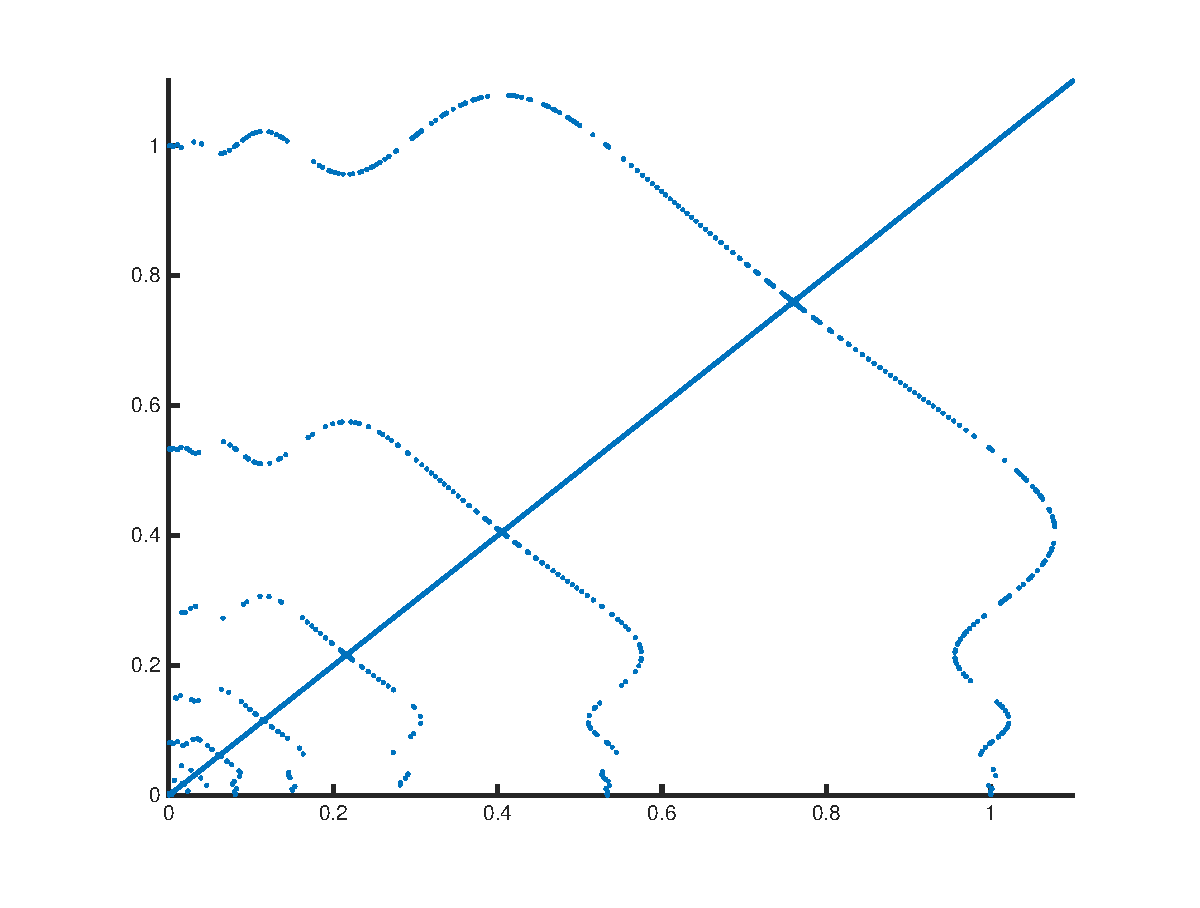
\includegraphics[width=10cm]{periodic/zeroset5}
\caption{Zero set of $H(a_0, a_1)$ for $\rho = 5$.}
\end{figure} 

In the next lemma, we show that pitchfork bifurcations occur on the diagonal in the zero set of $H(b_0, b_1)$ and identify their locations.

% lemma: pitchforks
\begin{lemma}\label{pitchforkH}
A discrete family of pitchfork bifurcations occurs along the diagonal in the zero set of $H(b_0, b_1)$ at 
\begin{align*}
(b_0, b_1) &= (p_k^*, p_k^*) && k \in \Z
\end{align*}
where 
\begin{equation}\label{pkstar}
p^*_k = \exp\left(-\frac{k \pi}{\rho} \right) p^*
\end{equation}
and 
\begin{equation}\label{pstar}
p^* = \exp \left( -\frac{1}{\rho} \arctan \rho \right)
\end{equation}
Locally, the arms of the pitchfork bifurcations open upwards along the diagonal.
\begin{proof}
First, we determine the locations of the pitchfork bifurcations along the diagonal. A necessary condition for these to occur is that the first derivative vanishes. The partial derivative of $H$ with respect to $b_0$ is
\begin{align*}
H_{b_0}(b_0, b_1) &= 
\sin \left( -\rho \log b_0 \right)
+ b_0 \cos \left( - \rho \log b_0 \right)- \rho \frac{1}{b_0} \\
&= \sin \left( - \rho \log b_0 \right) - \rho \cos \left( - \rho \log b_0 \right)
\end{align*}
Note that this does not depend on $b_1$. $H_{b_0}(b_0, b_1) = 0$ if and only if
\begin{align*}
\tan \left( -\rho \log b_0 \right) &=  \rho \\
-\rho \log b_0 &= \arctan \left( \rho\right) + k \pi && k \in \Z \\ 
b_0 &= \exp \left( -\frac{1}{\rho} \arctan \rho - \frac{k \pi}{\rho} \right) \\
&= \exp \left( -\frac{1}{\rho} \arctan \rho - \frac{k \pi}{\rho} \right)  \\
&= \exp \left( -\frac{1}{\rho} \arctan \rho \right) \exp \left( - \frac{k \pi}{\rho} \right) \\
&= p_k^*
\end{align*}

Next, we change coordinates so that the proposed pitchfork occurs along the $x$-axis. Let
\begin{align*}
x &= \frac{1}{2}(b_1 - b_0) \\
y &= \frac{1}{2}(b_1 + b_0)
\end{align*}
In terms of $b_0$ and $b_1$,
\begin{align*}
b_0 &= y - x \\
b_1 &= y + x
\end{align*}
Substituting these into $H(b_0, b_1)$ yields
\begin{equation}\label{Hxy}
H(x, y) = 
(y - x) \sin \left( -\rho \log(y - x) \right) - (y + x) \sin \left( - \rho \log (y + x) \right)
\end{equation}
We can see from \eqref{Hxy} that $H(-x, y) = -H(x, y)$, thus $H(x,y)$ has the required symmetry for a pitchfork bifurcation; $y$ will be the bifurcation parameter. In the $(x,y)$ coordinates, we expect the bifurcations to occur at $(x_0, y_0) = \left(0, p^*_k \right)$, where $k \in \Z$ is fixed.

To confirm this, we need to evaluate a series of partial derivatives at $(x_0, y_0)$. For the first derivatives,
\begin{align*}
H_x(x, y) &= -\sin \left( - \rho \log(y - x) \right) - 
\sin \left( - \rho \log(y + x) \right)
+\rho \cos \left( - \rho \log(y - x) \right) + \rho \cos \left( - \rho \log(y + x) \right) \\
H_y(x, y) &= \sin \left( - \rho \log(y - x) \right) - 
\sin \left( - \rho \log(y + x) \right)
-\rho \cos \left( - \rho \log(y - x) \right) + \rho \cos \left( - \rho \log(y + x) \right)
\end{align*}
Plugging in $(x_0, y_0) = \left(0, p^*_k \right)$ and noting that $\sin(\arctan \rho) = \rho / \sqrt{1 + \rho^2}$ and $\cos(\arctan \rho) = 1 / \sqrt{1 + \rho^2}$, we can see that both $H_x(x_0, y_0) = 0$ and $H_y(x_0, y_0) = 0$. 

Next, we look at the second partial derivatives. For $H_{xx}$, we have
\begin{align*}
H_{xx}(x, y) &= 
-(y-x) \left(-\frac{\rho^2 \sin \left(\rho \log (y-x)\right)}{(y-x)^2}-\frac{\rho
   \cos \left(\rho \log (y-x) \right)}{(y-x)^2}\right)\\
   &+(x+y) \left(-\frac{\rho^2
   \sin \left(\rho \log (x+y)\right)}{(x+y)^2}-\frac{\rho \cos \left( \rho
   \log (x+y)\right)}{(x+y)^2}\right)\\
   &-\frac{2 \rho \cos \left(\rho \log
   (y-x) \right)}{(y-x)}+\frac{2 \rho \cos \left( \rho \log (x+y) \right)}{
   (x+y)}
\end{align*}
After a tedious calculation, which can be verified by Mathematica, we conclude that $H_{xx}(x_0, y_0) = 0$. By symmetry, we also have $H_{yy}(x_0, y_0) = 0$. The mixed derivative $H_{xy}$ is
\begin{align*}
H_{xy}(x, y) &= -\frac{\rho^2 \sin \left(\rho \log (y-x)\right)}{(y-x)}-\frac{\rho^2 \sin
   \left(\rho \log (x+y)\right)}{(x+y)}+\frac{\rho \cos \left(\rho \log (y-x)\right)}{(y-x)}+\frac{\rho \cos \left( \rho \log (x+y) \right)}{(x+y)}
\end{align*}
Evaluating this at $(x_0, y_0) = \left(0, p^*_k \right)$, we have
\begin{align*}
H_{xy}(0, p^*_k) &= \frac{2 \rho}{p^*_k}\left( -\rho \sin \left(\rho \log p^*_k \right) + \cos \left(\rho \log p^*_k \right) \right)\\
&= \frac{2 \rho}{p^*_k}\left( -\rho \sin \left(\rho \log p^* + k \pi \right) + \cos \left(\rho \log p^* + k \pi \right) \right) \\
&= \frac{2 \rho}{p^*_k} (-1)^k \left( \rho \sin \left(\arctan \rho \right) + \cos \left(\arctan \rho \right) \right)\\ 
&= \frac{2 \rho}{p_n^*} (-1)^k \frac{\rho^2 + 1}{\sqrt{1 + \rho^2}} \\
&= (-1)^k 2 \rho \sqrt{1 + \rho^2} \: \exp{\left(\frac{1}{\rho} (\arctan \rho - k \pi) \right)}
\end{align*}
Since $\rho > 0$, this is nonzero. Let $c_1^k = H_{xy}(0, p^*_k)$. 

Finally, we check the third partial derivative with respect to $x$. This is another tedious calculation, but after substituting $(x_0, y_0) = \left(0, p^*_k \right)$ we obtain
\begin{align*}
H_{xxx}(0, p_k^*)
&= -(-1)^k 2 \rho \sqrt{1 + \rho^2} \: \exp{\left(\frac{2}{\rho} (\arctan \rho - k \pi) \right)}
\end{align*}
Since $\rho > 0$, this is also nonzero. Let $c_2^k = -H_{xxx}(0, p^*_k)$.

We have verified that a pitchfork bifurcation occurs at $(0, p^*_k)$ for $k \in \Z$. Near the bifurcation points $(0, p_k^*)$, we have the following Taylor expansions
\begin{align*}
H(x, y) &= c_1^k x (y - p_k^*) - \frac{c_2^k}{6} x^3 + \text{h.o.t.} \\
&= c_1^k x \left( (y - p_k^*) - \frac{c_2^k}{6 c_1^k } x^2 \right) + \text{h.o.t.} \\
&= c_1^k x \left( (y - p_k^*) - \frac{c_3^k}{6} x^2 \right) + \text{h.o.t.} \\
\end{align*}
where
\begin{equation*}
c_3^k = \exp{\left(\frac{1}{\rho} (\arctan \rho - k \pi) \right)} > 0
\end{equation*}
To leading order, the arms of the pitchforks are upwards-opening parabolas of the form 
\begin{align*}
y &= p_k^* + \frac{c_3^k}{6} x^2
\end{align*}
Since the above change of coordinates a rotation by $\pi/4$, we conclude that pitchfork bifurcations occur in the original coordinate system at $(b_0, b_1) = (p_k^*, p_k^*)$. Furthermore, the arms of the pitchforks are, to leading order, parabolas which open upwards along the diagonal.
\end{proof}
\end{lemma}

Now that we have located these pitchfork bifurcations, we will find a natural parameterization for the zero set of $H(b_0, b_1)$. Since the zero set is symmetric across the diagonal we only need to consider the case where $b_0 \geq b_1$. The parameterization works as follows. Recall that $H(b_0, b_1) = 0$ when $b_0, b_1 \in \mathcal{B}$; this is a discrete grid of points in the zero set of $H(b_0, b_1)$. We will then join these points with continuous curves parameterized by a phase parameter $\theta$. The specific form of the parameterization is given in the following lemma.

% lemma : parameterization of zero set of H

\begin{lemma}\label{thetaparamlemma}
Choose two baseline length parameters $b_0^0$ and $b_1^0$, where, $b_j^0 = \exp\left(-\frac{m_j \pi}{\rho}\right) \in \mathcal{B}$. Without loss of generality, take $b_0^0 \geq b_1^0$. (Alternatively, choose nonnegative integers $m_0$ and $m_1$, with $m_0 \leq m_1$). 

For every such choice, there is a smooth family of solutions $( b_0^*(m_0, \theta), b_1^*(m_1, \theta) )$ to $H(b_0, b_1) = 0$ parameterized by a phase parameter $\theta \in I_\rho$, with
\begin{equation}\label{Irho}
I_\rho = [\theta_\rho^-, \theta_\rho^+] = [-\arctan \rho,\pi - \arctan \rho] 
\end{equation}
and $(b_0^*(m_0, 0), b_1^*(m_1, 0)) = (b_0^0, b_1^0)$. In addition, we have the following properties.

\begin{enumerate}[(i)]
\item These families are disjoint except at their endpoints, where they connect as follows
\begin{align*}
\Big( b_0^*(m_0, \theta_\rho^-), b_1^*(m_1, \theta_\rho^-) \Big) &= \Big( b_0^*(m_0, \theta_\rho^+), b_1^*(m_1+1, \theta_\rho^+) \Big) \\
\Big( b_0^*(m, \theta_\rho^-), b_1^*(m, \theta_\rho^-) \Big) &= \Big( b_0^*(m+1, \theta_\rho^-), b_1^*(m+1, \theta_\rho^-) \Big) = \Big( b_0^*(m, \theta_\rho^+), b_1^*(m+1, \theta_\rho^+) \Big) = (p^*_m, p^*_m)
\end{align*}
where $(p^*_m, p^*_m)$ is the pitchfork bifurcation point from Lemma \ref{pitchforkH}.

\item The parameterization is given explicitly by
\begin{equation}\label{thetaparam}
\begin{aligned}
b_1^*(m_1, \theta) &= e^{-\frac{1}{\rho}(m_1 \pi - \theta) } \\
b_0^*(m_0, \theta) &= e^{-\frac{1}{\rho}(m_0 \pi - \theta_0^*(\theta)) }
\end{aligned}
\end{equation}
where $\theta_0^*(\theta) \in I_\rho$, and we have bound
\begin{equation}\label{thetastarbound}
|\theta_0^*(\theta)| \leq C e^{ -\frac{\pi}{\rho}(m_1 - m_0)}
\end{equation}
which is independent of $\theta$.
\end{enumerate}

\begin{proof}
First, we note that it suffices to consider the case where $b_0^0 = 1$, i.e. $m_0 = 0$. To see this, suppose the lemma is true for $b_0^0 = 1$. Then we can find a family of solutions $(b_0^*(0, \theta), b_1^*(m_1 - m_0, \theta))$ with $H(b_0, b_1) = 0$, where $m_1 - m_0 \geq 0$. Let 
\begin{equation}\label{btilde01}
\begin{aligned}
\tilde{b}_0(\theta) &= e^{-\frac{m_0 \pi}{\rho}} b_0^*(0, \theta) \\
\tilde{b}_1(\theta) &= e^{\frac{-m_0 \pi}{\rho}} b_1^*(m_1 - m_0, \theta).
\end{aligned} 
\end{equation}
Then since $\sin \left( -\rho \log ( e^{-m_0 \pi/\rho} x )\right) = (-1)^{m_0} \sin(-\rho \log x)$, 
\begin{align*}
H(\tilde{b}_0(\theta), \tilde{b}_1(\theta)) 
&= e^{-m_0 \pi/\rho} (-1)^m \Big( b_0^*(0, \theta) \sin (-\rho \log b_0^*(0, \theta)) - b_1^*(m_1 - m_0, \theta) \sin (-\rho \log b_1^*(m_1 - m_0, \theta))\Big) \\
&= e^{-m_0 \pi/\rho} (-1)^m H( b_0^*(0, \theta), b_1^*(m_1 - m_0, \theta)) \\
&= 0
\end{align*}
Thus $H(b_0, b_1) = 0$ for $(b_0, b_1) = (\tilde{b}_0(\theta), \tilde{b}_1(\theta))$, and 
\begin{align*}
\tilde{b}_0(\theta) &= e^{-m_0 \pi/\rho} b_0^*(0, 0) = b_0^0 \\
\tilde{b}_1(\theta) &= e^{-m_0 \pi/\rho} b_1^*(m_1 - m_0, 0) = b_0^1
\end{align*}

We may therefore take $b_0^0 = 1$. For $\theta \in I_\rho$, we will use the parameterization
\begin{equation}\label{thetaparam1}
\begin{aligned}
b_1^*(m_1, \theta) &= e^{ -\frac{1}{\rho}(m_1 \pi - \theta) } \\
b_0^*(0, \theta) &= e^{ \frac{1}{\rho} \theta_0^*(\theta) } \\
\end{aligned}
\end{equation}
where the function $\theta_0^*(\theta)$ will be determined below. It follows from this parameterization that $b_1^*(m_1, 0) = b_1^0$. Since we need to parameterize two pieces of a pitchfork, we will consider the cases $b_1^0 = 1$ and $b_1^0 > 1$ separately.

First, let $b_1^0 = 1$, so that $b_1^*(0, \theta) = e^{ \frac{1}{\rho}\theta}$. Then we can obtain a solution to $H(b_0, b_1) = 0$ by taking $\theta_0^*(\theta) = \theta$, so that $b_0^*(0, \theta) = e^{ \frac{1}{\rho}\theta}$, i.e. 
\[
( b_0^*(0, \theta), b_1^*(0, \theta) ) = ( e^{ \frac{1}{\rho}\theta }, e^{ \frac{1}{\rho}\theta })
\]
where $b_0 = b_1$, and $(b_0(0), b_1(0)) = (b_0^0, b_1^0) = (1,1)$. This parameterizes the center part of the pitchfork. We also note that
\begin{equation}\label{centerpitchforkparam}
\Big(b_0(0, \theta_\rho^-), b_1(0, \theta_\rho^-)\Big) = (p_0^*, p_0^*)
\end{equation}
where $p_0^*$ is the pitchfork bifurcation point defined in Lemma \ref{pitchforkH}.

Next, consider the case $b_1^0 \neq 1$ so that $m_1 > 0$. Plugging the expressions \eqref{thetaparam1} for $b_1^*(m_1, \theta)$ and $b_0^*(0, \theta)$ into $H$, we get
\begin{align*}
H(b_0, b_1) &= e^{ \frac{1}{\rho}\theta^* } \sin\left( -\rho \log e^{ \frac{1}{\rho}\theta^* }\right) - e^{ -\frac{1}{\rho}(m_1 \pi + \theta) }\sin \left( -\rho \log e^{ -\frac{1}{\rho}(m_1 \pi + \theta) } \right) \\
&= e^{ \frac{1}{\rho}\theta^* } \sin\left( -\theta^* \right) - e^{ -\frac{1}{\rho} m_1 \pi} e^{ \frac{1}{\rho} \theta } \sin(m_1 \pi - \theta) \\
&= -e^{ \frac{1}{\rho}\theta^* } \sin \theta^*  - e^{ -\frac{1}{\rho} m_1 \pi } e^{ \frac{1}{\rho} \theta } (-1)^{m_1 + 1} \sin\theta \\
&= -\left( e^{ \frac{1}{\rho}\theta^* } \sin \theta^* - e^{ -\frac{1}{\rho} m_1 \pi } (-1)^{m_1} e^{ \frac{1}{\rho} \theta } \sin \theta \right)
\end{align*}
Thus we need to solve the following equation for $\theta^*$.
\begin{align}\label{thetastareq}
e^{ \frac{1}{\rho}\theta^* } \sin\left( \theta^* \right) &= \left[ e^{ -\frac{1}{\rho} m_1 \pi } (-1)^{m_1} \right] e^{ \frac{1}{\rho} \theta } \sin(\theta)
\end{align}
where $\theta \in I_\rho$. We proceed in the following steps.
\begin{enumerate}
	\item Let $g(\theta) = e^{ \frac{1}{\rho} \theta } \sin(\theta)$. Then we can rewrite equation \eqref{thetastareq} as
	\begin{align}\label{thetastareq2}
	g(\theta^*) &= e^{ -\frac{1}{\rho} m_1 \pi } (-1)^{m_1} g(\theta)
	\end{align}
	First, we show that $g(\theta)$ is increasing on $I_\rho$. The derivative of $g$ is 
	\begin{equation}\label{gprime}
	g'(\theta) = e^{ \frac{1}{\rho} \theta } \left( \cos \theta + \frac{1}{\rho} \sin \theta \right)
	\end{equation}
	At the left endpoint of $I_\rho$,
	\begin{align*}
	g'(\theta_\rho^-) &= g'(-\arctan \rho) \\
	 &= e^{ -\frac{1}{\rho} \arctan \rho } \left(\cos(-\arctan \rho) + \frac{1}{\rho} \sin(-\arctan \rho)\right) \\
	&= e^{ -\frac{1}{\rho} \arctan \rho } \left(\cos\frac{1}{\sqrt{1 + \rho^2}} - \frac{1}{\rho} \frac{\rho}{\sqrt{1 + \rho^2}}\right) = 0
	\end{align*}
	Similarly, at the right endpoint of $I_\rho$, $g'(\theta_\rho^+) = 0$.
	The only critical point of $g'(\theta)$ on $I_\rho$ is a local maximum at $\theta = \arctan \rho$. Since $g'(\theta) > 0$ on the interior of $I_\rho$ and is zero at the endpoints, it follows that $g(\theta)$ is strictly increasing on $I_\rho$.
	
	\item It follows that the range of $g$ on $I_\rho$ is determined by the values of $g$ at the endpoints on $I_\rho$, thus for $\theta \in I_\rho$,
	\begin{equation}\label{grange}
	g(\theta) \in \left[ -\frac{\rho}{\sqrt{1+\rho^2}}e^{-\frac{1}{\rho}\arctan \rho}, \frac{\rho}{\sqrt{1+\rho^2}}e^{\frac{1}{\rho}(\pi - \arctan \rho)}\right] = [-T, e^{\frac{1}{\rho}\pi} T]
	\end{equation}
	where 
	\begin{equation}\label{defT}
	T = \frac{\rho}{\sqrt{1+\rho^2}}e^{-\frac{1}{\rho}\arctan \rho}
	\end{equation}
	Since $g$ is strictly increasing on $I_\rho$, $g$ is invertible on $[-T, e^{\frac{1}{\rho}\pi} T]$ and $g^{-1}: [-T, e^{\frac{1}{\rho}\pi} T] \rightarrow I_\rho$ is strictly increasing, with $g^{-1}(-T) = \theta_\rho^-$ and $g^{-1}(e^{\frac{1}{\rho}\pi} T) = \theta_\rho^+$.

	\item It follows from \eqref{grange} that the RHS of \eqref{thetastareq2} has bounds
	\begin{equation}\label{RHSbounds}
	e^{ -\frac{1}{\rho} m_1 \pi } (-1)^{m_1} g(\theta) \in
	\begin{cases}
	[-e^{-\frac{1}{\rho}m_1 \pi} T, e^{-\frac{1}{\rho}(m_1 - 1) \pi} T] & m_1 \text{ even }\\
	[-e^{-\frac{1}{\rho}(m_1 - 1) \pi} T, e^{-\frac{1}{\rho}m_1 \pi} T] & m_1 \text{ odd }
	\end{cases}
	\end{equation}
	Since $m_1 \geq 1$, 
	\begin{equation*}
	e^{ -\frac{1}{\rho} m_1 \pi } (-1)^{m_1} g(\theta) \in [-T, e^{\frac{1}{\rho}\pi} T]
	\end{equation*}
	Thus for $\theta \in I_\rho$, the RHS of \eqref{thetastareq2} is contained in the domain of $g^{-1}$, and so we solve for $\theta^*$ to get
	\begin{equation}\label{solvethetastar}
	\theta^* = g^{-1}\left( e^{ -\frac{1}{\rho} m_1 \pi } (-1)^{m_1}  e^{ \frac{1}{\rho} \theta } \sin \theta \right)
	\end{equation}
	It follows that $\theta^*(\theta) \in I_\rho$, which ensures that we cannot overlap the region parameterized by a different $b_0^0$ by varying $\theta$.

	\item For each $m_1$, equations \eqref{thetaparam1} and \eqref{solvethetastar} give us a smooth parameterization in $\theta$. We will now show that the pieces  match up. 

	First, we consider the case where $m_1 \geq 1$, so that we avoid the pitchfork bifurcation point $p_0^*$. Let $(b^*_0(0, \theta), b^*_1(m_1, \theta))$ and $(\tilde{b}^*_0(0, \theta), \tilde{b}^*_1(m_1 + 1, \theta))$ parameterize adjacent pieces. For the second component,
	\begin{align*}
	b_1^*(m_1, \theta_\rho^-) &= e^{ -\frac{1}{\rho}(m_1 \pi + \arctan \rho) }
	\end{align*}
	and
	\begin{align*}
	\tilde{b}_1^*(m_1 + 1, \theta_\rho^+) 
	&= e^{ -\frac{1}{\rho}((m_1+1) \pi - (\pi - \arctan \rho)) } \\
	&= e^{ -\frac{1}{\rho}(m_1 \pi + \arctan \rho) }
	\end{align*}
	Thus the second components match. For the first component, let $b_0^*(0, \theta) = e^{ \frac{1}{\rho} \theta_0^*(\theta) }$ and $\tilde{b}_0^*(0, \theta) = e^{ \frac{1}{\rho} \tilde{\theta}_0^*(\theta) }$. From \eqref{solvethetastar}, $\theta_0^*$ and $\tilde{\theta}_0^*$ are given by
	\begin{align*}
	\theta_0^* &= g^{-1}\left( e^{ -\frac{1}{\rho} m_1 \pi } (-1)^{m_1}  e^{ -\frac{1}{\rho} \arctan \rho } \sin(-\arctan \rho) \right)
	\end{align*}
	and
	\begin{align*}
	\tilde{\theta}_0^* &= g^{-1}\left( e^{ -\frac{1}{\rho} (m_1+1) \pi } (-1)^{m_1+1}  e^{ \frac{1}{\rho} (\pi - \arctan \rho) } \sin(\pi - \arctan \rho) \right) \\
	&= g^{-1}\left( e^{ -\frac{1}{\rho} m_1 \pi } (-1)^{m_1+1} e^{-\frac{1}{\rho} \arctan \rho } (-1) \sin(- \arctan \rho) \right) \\
	&= g^{-1}\left( e^{ -\frac{1}{\rho} m_1 \pi } (-1)^{m_1} e^{-\frac{1}{\rho} \arctan \rho } \sin(-\arctan \rho) \right)
	\end{align*}
	Since the RHS of the two equations is the same, $\theta_0^* = \tilde{\theta}_0^*$, thus the first components match as well.

	\item We showed in \eqref{centerpitchforkparam} that for $m_1 = 0$, we hit the pitchfork bifurcation point at $\theta = \theta_\rho^-$. Next, we show that for $m_1 = 1$, we hit the pitchfork bifurcation point $p_0^*$ at $\theta = \theta_\rho^+$. 
	For the second component, 
	\begin{align*}
	b_1^*(1, \theta_\rho^+) &= e^{-\frac{1}{\rho}(\pi - (\pi - \arctan \rho)) } \\
	&= e^{ -\frac{1}{\rho} \arctan \rho } \\
	&= p_0^*
	\end{align*}
	For the first component, for $\theta = \theta_\rho^+ = \pi -\arctan \rho$, the RHS of \eqref{thetastareq} is $-T$, thus $\theta_0^* = g^{-1}(-T) = -\arctan \rho$, and so 
	\[
	b_0^*(1, \theta_\rho^+) = e^{ \frac{1}{\rho} \theta_0^*(\theta_\rho^+)} = e^{ -\frac{1}{\rho} \arctan \rho } = p_0^*
	\]
	Thus $(b_0^*(0, \theta_\rho^+), b_1^*(1, \theta_\rho^+)) = (p_0^*,p_0^*).$

	\item Finally, we will obtain a bound for $\theta_0^*(\theta)$. This will be in terms of $m_1$. From \eqref{RHSbounds},
	\begin{equation}\label{easyRHSbound}
	|e^{ -\frac{1}{\rho} m_1 \pi } (-1)^{m_1 + 1} g(\theta)| \leq C e^{ -\frac{1}{\rho}(m_1 - 1) \pi }
	\end{equation}
	Since $g(0) = 0$ and $g^{-1}$ is smooth, $\theta^* \rightarrow 0$ as $m_1 \rightarrow \infty$. From \eqref{gprime}, we have $g'(0) = 1$. To get a decay rate, we first note that
	\begin{align*}
	(g^{-1})'(0) &= \frac{1}{g'(g^{-1}(0))} \\
	&= \frac{1}{g'(0)} \\
	&= 1
	\end{align*}
	Since $g^{-1}$ is smooth, we can find a neighborhood $[-R, R]$ of 0 contained in the domain of $g^{-1}$ such that $|(g^{-1})'(\theta)| \leq 2$ on $[-R, R]$. Using \eqref{easyRHSbound}, we can find an integer $M_1$ such that for $m_1 \geq M_1$ and $\theta \in I_\rho$,
	\begin{equation}\label{easyRHSbound2}
	|e^{ -\frac{1}{\rho} m_1 \pi } (-1)^{m_1 + 1} g(\theta)| \leq R
	\end{equation}
	Thus, by the mean value theorem and \eqref{easyRHSbound2}, for $m_1 \geq M_1$ and $\theta \in I_\rho$,
	\begin{align*}
	|\theta_0^*(\theta)| &= | g^{-1}(e^{ -\frac{1}{\rho} m_1 \pi } (-1)^{m_1 + 1} g(\theta) | \\
	&\leq 2 |e^{ -\frac{1}{\rho} m_1 \pi } (-1)^{m_1 + 1}  e^{ \frac{1}{\rho} \theta } \sin(\theta)| \\
	&\leq C e^{ -\frac{1}{\rho}(m_1 - 1) \pi } \\
	&\leq C e^{ -\frac{\pi}{\rho} m_1 }
	\end{align*}
	If $m_0 > 0$, we multiply this bound by $e^{m_0 \pi/\rho}$.
\end{enumerate}
\end{proof}
\end{lemma}

In the final lemma of this section, we obtain bounds on the partial derivative $H_{b_0} (b_0, b_1)$ on the zero set of $H$, where we parameterize this zero set according to Lemma \ref{thetaparamlemma}.

% derivative bounds

\begin{lemma}\label{Hderivboundslemma}
Fix $m_0 \in \N_0$. For each integer $m_1$ with $m_1 \geq m_0$, let $(b_0^*(m_0, \theta), b_1^*(m_1, \theta))$ be the parameterization of the appropriate piece of the zero set of $H$ according to Lemma \ref{thetaparam}. 

Then for any $\delta > 0$, there exists $\eta > 0$ depending on $\delta$ such that if either $m_1 \geq 2$ and $\theta \in I_\rho$ or $m_1 = 1$ and $\theta \in [\theta_\rho^-, \theta_\rho^+ - \delta]$,
\begin{align}\label{Hderivbound}
| H_{b_0}(b_0^*(m_0, \theta), b_1^*(m_1, \theta)) | &\geq \eta
\end{align}

\begin{proof}
From Lemma \ref{thetaparamlemma}, $b_0^*(m_0, \theta)$ is given by
\begin{align}\label{b0starexp}
b_0^*(m_0, \theta) &= e^{-\frac{1}{\rho}(m_0 \pi - \theta_0^*(\theta)) }
\end{align}
where $|\theta_0^*(\theta)| \leq C e^{ -\frac{\pi}{\rho}(m_1 - m_0)}$.

The partial derivative of $H(b_0, b_1)$ with respect to $b_0$ is
\begin{align}\label{Hb0}
H_{b_0} (b_0, b_1) = \sin(-\rho \log b_0) - \rho \cos(-\rho \log b_0)
\end{align}
Evaluating this at $(b_0, b_1) = (b_0^*(m_0, \theta), b_1^*(m_1, \theta))$, 
\begin{align*}
H_{b_0}(b_0^*(m_0, \theta), b_1^*(m_1, \theta)) &= \sin\left(-\rho \log e^{-\frac{1}{\rho}(m_0 \pi - \theta_0^*(\theta))} \right) - \rho \cos\left(-\rho \log e^{-\frac{1}{\rho}(m_0 \pi - \theta_0^*(\theta))} \right) \\
&= \sin\left(m_0 \pi - \theta_0^*(\theta) \right) - \rho \cos\left(m_0 \pi - \theta_0^*(\theta) \right) \\
&= -(-1)^{m_0} \sin \theta_0^*(\theta) - \rho (-1)^{m_0} \cos \theta_0^*(\theta) \\
&= (-1)^{m_0+1} \left( \sin \theta_0^*(\theta) + \rho \cos \theta_0^*(\theta) \right)
\end{align*}

Recall from the proof of Lemma \ref{thetaparamlemma} that we found $\theta_0^*$ by solving
\begin{equation*}
\theta_0^* = g^{-1}\left( e^{ -\frac{1}{\rho} m_1 \pi } (-1)^{m_1} g(\theta) \right)
\end{equation*}
where $g(\theta) = e^{ \frac{1}{\rho} \theta } \sin \theta$. For $m_1 \geq 2$ and $\theta \in I_\rho$, we have from \eqref{RHSbounds},
\begin{align}\label{RHSboundgeq2}
e^{ -\frac{1}{\rho} m_1 \pi } (-1)^{m_1} g(\theta) \in [-e^{ -\frac{1}{\rho} \pi } T, e^{ -\frac{1}{\rho} \pi } T]
\end{align}
where
\begin{equation*}
T = \frac{\rho}{\sqrt{1+\rho^2}}e^{-\frac{1}{\rho}\arctan \rho}
\end{equation*}

For $m = 1$, we would like to exclude a small neighborhood of the pitchfork bifurcation point. For any $\delta > 0$, let $I_\rho(\delta) = [-\theta_\rho^-, \theta_\rho^+ - \delta]$. From Lemma \ref{thetaparamlemma}, $g(\theta)$ is strictly increasing on $I_\rho$, thus for $\theta \in I_\rho(\delta)$,
\begin{align*}
-e^{ -\frac{1}{\rho} \pi } g(\theta) &\geq 
 -e^{ -\frac{1}{\rho} \pi } e^{ \frac{1}{\rho}(\pi - \arctan \rho - \delta) } \sin(\pi - \arctan \rho - \delta) \\
&= -e^{-\frac{1}{\rho}\delta} e^{-\frac{1}{\rho}\arctan\rho}\sin(\arctan \rho - \delta) \\
&\geq -e^{-\frac{1}{\rho}\delta} e^{-\frac{1}{\rho}\arctan\rho}\sin(\arctan \rho)
\end{align*}
since $0 < \arctan \rho < \pi/2$. Evaluating $\sin(\arctan\rho)$ and simplifying, this becomes
\begin{align*}
-e^{ -\frac{1}{\rho} \pi } g(\theta)
&\geq -e^{-\frac{1}{\rho}\delta} e^{-\frac{1}{\rho}\arctan\rho}\frac{\rho}{\sqrt{1 + \rho^2}} \\
&= -e^{-\frac{1}{\rho}\delta} T
\end{align*}

Thus for $m = 1$ and $\theta \in I_\rho(\delta)$, we have
\begin{align*}
-e^{ -\frac{1}{\rho} \pi } g(\theta)
\in [-e^{-\frac{1}{\rho}\delta} T, e^{ -\frac{1}{\rho} \pi } T]
\end{align*}
Since the interval in \eqref{RHSboundgeq2} is contained in this interval, we conclude that if either $m_1 \geq 2$ and $\theta \in I_\rho$ or $m_1 = 1$ and $\theta \in I_\rho(\delta)$,
\begin{align}\label{RHSbound2}
e^{ -\frac{1}{\rho} m_1 \pi } (-1)^{m_1} g(\theta) \in [-e^{-\frac{1}{\rho}\delta} T, e^{ -\frac{1}{\rho} \pi } T]
\end{align}
From Lemma \ref{thetaparamlemma}, $g^{-1}$ is strictly increasing on $[-T,e^{\frac{1}{\rho}\pi}T]$, and at the endpoints of its domain, $g^{-1}(-T) = \theta_\rho^+$ and $g^{-1}(e^{\frac{1}{\rho}\pi}T) = \theta_\rho^+$. Since $e^{-\frac{1}{\rho} m_1 \pi } (-1)^{m_1} g(\theta)$ lies strictly inside these endpoints, we conclude that there exists $\epsilon > 0$ (depending on $\delta$) such that 
\begin{equation}\label{thetastarboundeps}
\theta_0^*(\theta) \in [\theta_\rho^- + \epsilon, \theta_\rho^+ - \epsilon]
\end{equation}
Using this bound together with \eqref{b0starexp},
\begin{align*}
b_0^*(m_0, \theta) 
&\in \left[e^{-\frac{1}{\rho}(m_0 \pi - (\theta_\rho^- + \epsilon)) }, e^{-\frac{1}{\rho}(m_0 \pi - (\theta_\rho^+ - \epsilon)) }\right] \\
&= \left[ e^{-\frac{1}{\rho} m_0 \pi} e^{-\frac{1}{\rho} (\arctan \rho - \epsilon)}, e^{-\frac{1}{\rho} m_0 \pi} e^{-\frac{1}{\rho} (\arctan \rho - \pi + \epsilon)}\right] \\
&= \left[ e^{-\frac{1}{\rho} m_0 \pi} e^{-\frac{1}{\rho} \arctan \rho} e^{\frac{1}{\rho}\epsilon}, e^{-\frac{1}{\rho} (m_0-1) \pi} e^{-\frac{1}{\rho} \epsilon}\right] \\
&= \left[ e^{\frac{1}{\rho}\epsilon} p_{m_0}^*, e^{-\frac{1}{\rho} \epsilon} p_{m_0 + 1}^* \right]
\end{align*}

From the proof of Lemma \ref{pitchforkH}, $H_{b_0}(b_0, b_1)$ is smooth and is 0 if and only if $b_0 = p_k^*$ for some $k \in \Z$. Since the closed interval $\left[ e^{\frac{1}{\rho}\epsilon} p_{m_0}^*, e^{-\frac{1}{\rho} \epsilon} p_{m_0 + 1}^* \right]$ lies strictly inside the interval $[p_{m_0}^*, p_{m_0+1}^*]$, there exists $\eta > 0$ (which depends on $\epsilon$, thus on $\delta$) such that if either $m_1 \geq 2$ and $\theta \in I_\rho$ or $m_1 = 1$ and $\theta \in I_\rho(\delta)$
\[
|H_{b_0} (b_0^*(m_0, \theta), b_1^*(m_1, \theta))| \geq \eta
\]
\end{proof}
\end{lemma}

Now that we have our parameterization for $r = 0$, we would like to use it to solve \eqref{Geq} for small $r$. When we perturb $r$ away from 0, we will generically lose the pitchfork bifurcation structure. In addition, since this relies on the implicit function theorem, we will not be able to perturb $r$ at the pitchfork bifurcation points. In the next two sections, we prove the existence theorems for periodic multi-pulses. After that, we will show that in the special case of the 2-periodic pulse, the entire bifurcation structure of $H$ persists for small $r$.

\subsection{Proof of Theorem \ref{Pi:perexist}}

By Lemma \ref{diagonalG}, a periodic $n-$pulse exists if and only if the $n-1$ jump conditions
\begin{align}\label{Geq2}
G_j(b_0, \dots, b_{n-1}, r) = b_j \sin \left( -\rho \log b_j \right) - b_{n-1} \sin \left( -\rho \log b_{n-1} \right) + \mathcal{O}(r^{\gamma / 2 \alpha}) &= 0 && i = 0, \dots, n-2
\end{align}
are satisfied. For $r = 0$, $G_j(b_0, \dots, b_{n-1}, 0) = H(b_j, b_{n-1})$, and we can parameterize the zero set of $H$ using Lemma \ref{thetaparamlemma}. 

Since we are on a periodic domain, we can without loss of generality choose $b_{n-1}^0 \leq b_j^0$ (equivalently $m_{n-1} \geq m_j$) for $j = 0, \dots, n-2$. Using Lemma \ref{thetaparamlemma}, 
\begin{align*}
(b_j^*(m_0, \theta), b_{n-1}^*(m_{n-1}, \theta)) && j = 0, \dots, n-2
\end{align*}
be the families of solutions to $H(b_i, b_{n-1}) = 0$ with $b_j^*(m_j, 0) = b_j^0$, where $\theta \in [-\arctan \rho, \pi - \arctan \rho)$. Since for all of these families, $b_{n-1}^*(m_{n-1}, \theta)$ is given by
\begin{equation}\label{bstarlast}
b_{n-1}^*(m_{n-1}, \theta) = e^{-\frac{1}{\rho}(m_{n-1}\pi - \theta)}
\end{equation}
these are well-defined. 

Taking $b_{n-1} = b_{n-1}^*(m_{n-1}, \theta)$ in \eqref{Geq2}, define $G: \R^{n-1} \times \mathcal{R} \rightarrow \R^{n-1}$ by $G = (G_0, \dots, G_{n-2})^T$, where 
\begin{equation*}
G_j(b, r) = b_j \sin \left( -\rho \log b_j \right) - b_{n-1}^*(m_{n-1}, \theta) \sin \left( -\rho \log b_{n-1}^*(m_{n-1}, \theta) \right) + \mathcal{O}(r^{\gamma / 2 \alpha})
\end{equation*}
where $b = (b_0, \dots, b_{n-1})$. Note that $b_{n-1} = b_{n-1}^*(m_{n-1}, \theta)$ is fixed in these equations and that $G(b^*, 0) = 0$,
where
\[
b^*(\theta) = \left( b_1^*(m_1, \theta), \dots, b_{n-2}^*(m_{n-2}, \theta) \right)
\]

Next, we evaluate the partial derivatives of $G_k$ with respect to $b_j$. For $j \neq k$, 
\[
\partial_{b_j} G_k(b, r) = \mathcal{O}(r^{\gamma/2\alpha})
\]
where the order of the remainder term comes from Lemma \ref{jumplemma3}. For $j = k$, 
\begin{align*}
\partial_{b_j} G_j(b, r) &= 
\sin \left( -\rho \log b_j \right) - \rho b_j \cos \left( -\rho \log b_j \right) \frac{1}{b_j} + \mathcal{O}(r^{\gamma/2\alpha}) \\
&= \sin \left( -\rho \log b_j \right) - \rho \cos \left( -\rho \log b_j \right) + \mathcal{O}(r^{\gamma/2\alpha}) 
\end{align*}
where the order of the remainder term again comes from Lemma \eqref{jumplemma3}. Evaluating these at $r = 0$ and $b = b^*(\theta)$, the Jacobian matrix $D_b G(b^*(\theta),0)$ is diagonal, with the diagonal entries given by 
\begin{align*}
\partial_{b_j} G_j(b^*(\theta), 0)
&= \sin \left( -\rho \log b_j^*(m_j, \theta) \right) - \rho \cos \left( -\rho \log b_j^*(m_j, \theta) \right)
\end{align*}

We can use the implicit function theorem as long these partial derivatives are nonzero. From Lemma \ref{pitchforkH}, $\partial_{b_j} G_j(b, 0) = 0$ if and only if $b_j = p_k^*$, where $p_k^*$ is one of the pitchfork bifurcation points in the zero set of $H$. From Lemma \ref{thetaparamlemma}, this can only occur if for some $j$ either of the following is true.
\begin{itemize}
\item $m_j = m_{n-1}$ and $\theta = -\arctan \rho$
\item $m_j = m_{n-1} - 1$ and $\theta = \pi-\arctan \rho$
\end{itemize}

As long as we avoid these parameter values, $D_b G(b^*(\theta), 0)$ is invertible. Thus, for sufficiently small $r$, we can use the IFT to solve for $b$ in terms of $r$ near $b^*(\theta)$. Specifically, there exists $r_0 > 0$ and a smooth function $b: \mathcal{R} \cap [0, r_0] \rightarrow \R^{n-1}$ such that $b(0) = b^*(\theta)$ and $G(b(r),r) = 0$. Writing $b$ in terms of its component functions as
\[
b(r) = \left( b_0(r; m_0, \theta), \dots, b_{n-2}(r; m_{n-2}, \theta) \right)
\]
we have $b_j(0; m_j, \theta) = b_j^*(m_j, \theta)$. Since we have satisfied the $n-1$ jump conditions, we have successfully constructed a periodic $n-$pulse solution. 

Uniqueness comes from the fact that the solution families $(b_j^*(m_0, \theta), b_{n-1}^*(m_{n-1}, \theta))$ from Lemma \eqref{thetaparamlemma} only overlap at the endpoints. We are avoiding that overlap by taking $\theta$ in the half-open interval $[-\arctan \rho, \pi - \arctan \rho)$. 

\subsection{Proof of Theorem \ref{Pi:unifperexist}}

We parameterize the zero set of $H$ as in Lemma \ref{thetaparamlemma}, but this time we take $m_{n-1}$ to be an additional parameter. Fix baseline length parameters $\{ b_0^0, \dots, b_{n-2}^0 \}$, where $b_j^0 = \exp(-\frac{1}{\rho}m_j \pi) \in \mathcal{B}$, with the restriction that at least one of them must be 1. Let $b^0 = (b_0^0, \dots b_{n-2}^0)$.

Let $m = \max\{ m_0, \dots, m_{n-2} \}$. For each $m_{n-1} \geq m$ let
\begin{align}
(b_j^*(m_0, \theta; m_{n-1}), b_{n-1}^*(m_{n-1}, \theta)) && j = 0, \dots m_{n-2}
\end{align}
be the family of solutions to $H(b_j, b_{n-1}) = 0$, where $\theta \in [-\arctan \rho, \pi - \arctan \rho)$. From Lemma \ref{thetaparamlemma}, these are given by
\begin{equation}\label{bstarm}
\begin{aligned}
b_j^*(m_j, \theta; m_{n-1}) &= e^{-\frac{1}{\rho}(m_j \pi - \theta_j^*(\theta; m_{n-1}))} && j = 0, \dots, n-2 \\
b_{n-1}^*(m_{n-1}, \theta) &= e^{-\frac{1}{\rho}(m_{n-1}\pi - \theta)}
\end{aligned}
\end{equation}
Since for a given $m_{n-1}$, $b_{n-1}^*(m_{n-1}, \theta)$ is the same for each $j$, these are well-defined. Finally, let
\begin{equation}\label{defbstar}
b^*(\theta, m_{n-1}) = 
\left( b_0^*(m_0, \theta; m_{n-1}), \dots, b_{n-2}^*(m_{n-2}, \theta; m_{n-1}) \right)
\end{equation}

As in the proof of Theorem \ref{Pi:perexist}, we plug $b_{n-1}^*(m_{n-1}, \theta)$ into \eqref{Geq}. This time, however, we leave $m_{n-1}$ and $\theta$ as parameters. Define the map $G: \R^{n-1} \times \N \cap [m, \infty) \times I_\rho \times \mathcal{R} \rightarrow \R^{n-1}$ by $G = (G_0, \dots, G_{n-2})^T$, where 
\begin{equation}\label{Gdef2}
G_j(b, m_{n-1}, \theta, r) = b_j \sin \left( -\rho \log b_j \right) - b_{n-1}^*(m_{n-1}, \theta) \sin \left( -\rho \log b_{n-1}^*(m_{n-1}, \theta) \right) + \mathcal{O}(r^{\gamma / 2 \alpha})
\end{equation}
where $b = (b_0, \dots, b_{n-2})$. Then for all $m_{n-1} \geq m$ and $\theta \in I_\rho$, $G(b^*(\theta, m_{n-1}), m_{n-1}, \theta, 0) = 0$.

Next, we evaluate the Jacobian matrix $D_b G(b^0, m_{n-1}, \theta, 0)$. As in the proof of the previous theorem, $\partial_{b_j} G_k(b, m_{n-1}, \theta, 0) = 0$ for $j \neq k$. For $j = k$,
\begin{align*}
\partial_{b_j} G_j(b, m_{n-1}, \theta, 0) &= \sin \left( -\rho \log b_j \right) - \rho \cos \left( -\rho \log b_j \right) 
\end{align*}
which involves neither $m_{n-1}$ nor $\theta$. Evaluating this at $b^0$,
\begin{align*}
\partial_{b_j} G_j(b^0, m_{n-1}, \theta, 0) &= \sin \left( -\rho \log b_j^0 \right) - \rho \cos \left( -\rho \log b_j^0 \right) \\
&= \sin \left( m_j \pi \right) - \rho \cos \left(m_j \pi \right) \\
&= (-1)^{m_j + 1} \rho
\end{align*}
Thus $D_b G(b^0, m_{n-1}, \theta, 0)$ is diagonal with entries $\{ (-1)^{m_0 + 1} \rho, \dots, (-1)^{m_{n-2} + 1} \rho \}$. This implies that $D_b G(b^0, m_{n-1}, \theta, 0)$ is invertible, and the inverse has bound
\begin{equation}\label{DbG0invbound}
||D_b G(b^0, m_{n-1}, \theta, 0)^{-1}|| \leq \frac{1}{\rho}
\end{equation}

We can use the uniform contraction mapping principle to solve for $b$ in terms of $r$ near $b^*(\theta, m_{n-1})$. Specifically, define the map $K: \R^{n-1} \times \N \cap [m, \infty) \times I_\rho \times \mathcal{R} \rightarrow \R^{n-1}$ by
\begin{equation}\label{defKb}
K(b, m_{n-1}, \theta, r) = b - [D_b G(b^0, m_{n-1}, \theta, 0)]^{-1} G(b, m_{n-1}, \theta, r)
\end{equation}
$K(b, m_{n-1}, \theta, r) = b$ if and only if $G(b, m_{n-1}, \theta, r) = 0$. In particular, $K(b^*(\theta, m_{n-1}), m_{n-1}, \theta, 0) = b^*(\theta, m_{n-1})$. Since $G$ is smooth, so is $K$, and 
\begin{equation}\label{DbK}
D_b K(b, m_{n-1}, \theta, r) = I - [D_b G(b^0, m_{n-1}, \theta, 0)]^{-1} D_b G(b, m_{n-1}, \theta, r)
\end{equation}
In particular, $D_b K(b^0, b_{n-1}, \theta, 0) = 0$.

First, we obtain a bound for $D_b K(b, m_{n-1}, \theta, r)$ in a neighborhood of $b^0$. Let $U_0(\delta)$ be the open ball of radius $\delta$ about $b^0$ in $\R^{n-1}$. Since $K$ is smooth in $b$ and $r$, we can find $r_1 > 0$ and $\delta > 0$ such that for all $r < r_1$ and $b \in \overline{ U_0(\delta) }$,  
\begin{align}\label{DbKbound}
|| D_b K(b, m_{n-1}, \theta, r)|| \leq \frac{1}{2}
\end{align}
Since $D_b K(b, m_{n-1}, \theta, r)$ does not involve $m_{n-1}$ and $\theta$, this bound is independent of these parameters.

Next, we obtain a bound for $G(b^0, b_{n-1}, \theta, r)$. Taking $b = b^0$ and $b_{n-1} = b_{n-1}^*(m_{n-1}, \theta)$ in \eqref{Gdef2},
\begin{align*}
G_j(b^0, m_{n-1}, \theta, r) &= e^{-\frac{1}{\rho}m_j \pi} \sin \left( -\rho \log e^{-\frac{1}{\rho}m_j \pi} \right) - e^{-\frac{1}{\rho}(m_{n-1}\pi - \theta)} \sin \left( -\rho \log e^{-\frac{1}{\rho}(m_{n-1}\pi - \theta)} \right) + \mathcal{O}(r^{\gamma / 2 \alpha}) \\
&= e^{-\frac{1}{\rho}m_j \pi} \sin \left( m_j \pi \right) - e^{-\frac{1}{\rho} m_{n-1}\pi } e^{\frac{1}{\rho}\theta } \sin \left(m_{n-1} \pi - \theta \right) + \mathcal{O}(r^{\gamma / 2 \alpha}) \\
&= -e^{-\frac{1}{\rho} m_{n-1}\pi } e^{\frac{1}{\rho}\theta } \sin \left(m_{n-1} \pi - \theta \right) + \mathcal{O}(r^{\gamma / 2 \alpha}) \\
&= e^{-\frac{1}{\rho} m_{n-1}\pi } (-1)^{m_{n-1}} e^{\frac{1}{\rho}\theta } \sin \theta + \mathcal{O}(r^{\gamma / 2 \alpha}) \\
\end{align*}
Since the first term on the RHS decays exponentially in $m_{n-1}$, we can find $M_0 \geq m$ and decrease $r_1$ (if necessary) so that for all $r \leq r_1$ and $m_{n-1} \geq M_0$,
\begin{align}\label{G0bound}
|G(b^0, m_{n-1}, \theta, r)| \leq \frac{\delta \rho}{2}
\end{align}

Finally, using the parameterization \eqref{bstarm}, for $j = 0, \dots, n-2$,
\begin{align*}
| b_j^*(m_j, \theta; m_{n-1}) - b_j^0| &=
| e^{-\frac{1}{\rho}(m_j \pi - \theta_j^*(\theta; m_{n-1}))} - b_j^0 | \\
&= e^{-\frac{1}{\rho}m_j \pi}| 1 - e^{\frac{1}{\rho} \theta_j^*(\theta; m_{n-1})}| 
\end{align*}
Using \eqref{thetastarbound} from Lemma \ref{thetaparamlemma}, $\theta_j^*(\theta; m_{n-1}) \rightarrow 0$ as $m_{n-1} \rightarrow \infty$. Thus we can find $M_1 \geq M_0$ such that for all $m_{n-1} \geq M_1$ and $\theta \in I_\rho$, $|b^*(\theta, m_{n-1}) - b^0| \leq \delta$. Let $\mathcal{N} = \{ m \in \N : m \geq M_1 \}$.

Using the bounds \eqref{DbKbound} and \eqref{G0bound}, for all $b \in \overline{U_0(\delta)}$ and $r \leq r_1$
\begin{align*}
|K(b, &m_{n-1}, \theta, r) - b^0| \\
&\leq |K(b, m_{n-1}, \theta, r) - K(b^0, m_{n-1}, \theta, r)| + |K(b^0, m_{n-1}, \theta, r) - b^0| \\ 
&\leq \sup_{b\in \overline{U_0(\delta)}}||D_b K(b, m_{n-1}, \theta, r)||\:|b - b^0| 
+ || [D_b G(b^0, m_{n-1}, \theta, 0)]^{-1} G(b^0, m_{n-1}, \theta, r) || \\
&< \frac{1}{2} |b - b^0| + \frac{1}{\rho} ||G(b^0, b_{n-1}, \theta, r) ||  \\
&\leq \frac{\delta}{2} + \frac{1}{\rho}\frac{\delta \rho}{2} \\
&\leq \delta
\end{align*} 

Thus we have shown $K: \overline{U_0(\delta)} \times \mathcal{N} \times I_\rho \times \mathcal{R} \cap [0, r_1] \rightarrow \overline{U_0(\delta)}$, where $\overline{U_0(\delta)}$ is a closed subset of a complete metric space. To show that $K$ is a uniform contraction, let $b, \tilde{b} \in \overline{U_0(\delta)}$ and $r \leq r_1$. Then for any $m_{n-1} \in \mathcal{N}$ and $\theta \in I_\rho$,
\begin{align*}
|H(b, m_{n-1}, \theta, r) - H(\tilde{b}, m_{n-1}, \theta, r)| 
&\leq \sup_{b\in \overline{U_0}}||D_b H(b, b_{n-1}, \theta, r)||\:|b - \tilde{b}| \\
&\leq \frac{1}{2} |b - \tilde{b}|
\end{align*} 

Thus we can use the uniform contraction mapping principle to conclude that there is a unique smooth function $b: \mathcal{R} \cup [0, r_1] \times \mathcal{N} \times I_\rho \rightarrow \overline{U_0(\delta)}$ which maps $r \in \mathcal{R}$ with $r \leq r_1$ to the unique fixed point $b$ of $K(\cdot, m_{n-1}, \theta, r)$. By uniqueness, $b(0, m_{n-1}, \theta) = b^*(\theta, m_{n-1})$. Thus for $r \leq r_1$, $m_{n-1} \in \mathcal{N}$, and $\theta \in I_\rho$,
\[
G(b(r, b_{n-1}, \theta), b_{n-1}, \theta, r) = 0
\]
By uniqueness, all solutions obtained this way must be identical to the solutions obtained using Theorem \ref{Pi:perexist} using the corresponding set of parameters.

\subsection{2-periodic pulse}
In the special case of the 2-periodic pulse, we will be able to provide the complete bifurcation structure for sufficiently small $r$. For the 2-periodic pulse, by Lemma \ref{jumplemma3}, we only have one equation to solve
\begin{equation}\label{2pulsedefG}
G(b_0, b_1, r) = b_0 \sin \left( -\rho \log b_0 \right) - b_1 \sin \left( -\rho \log b_1 \right) + \mathcal{O}(r^{\gamma / 2 \alpha}) = 0 \\
\end{equation}
where, for convenience, we have dropped the subscript on $G$.

First, we will show that the pitchfork bifurcation persists for small $r$. In the first lemma, we show that $G$ has the same symmetries as $H$.

% lemma : symmetries of G
\begin{lemma}\label{Gsymm}
For sufficiently small $r$, we have the symmetry relation
\begin{equation}
G(b_0, b_1, r) = -G(b_1, b_0, r)
\end{equation}
In particular, 
\[
G(b_0, b_0, r) = 0
\]
\begin{proof}
In Lemma \ref{solvewithjumps}, we showed that given sufficiently large lengths $X_0$ and $X_1$ (i.e. sufficiently small $r$), there exists a unique piecewise solution $\{ U_0^-(x), U_0^+(x), U_1^-(x), U_1^+(x) \}$ to \eqref{systemwithjumpZ} which generically has two jumps at $x = 0$ in the direction of $\Psi(0)$. A periodic 2-pulse solution exists if and only if these jumps are 0. By uniqueness, these jumps are functions of $X_0$ and $X_1$ and are given by
\begin{equation}\label{xijumps}
\begin{aligned}
\xi_0(X_0, X_1) &= \langle \Psi(0), U_0^+(0) - U_0^-(0) \rangle  \\
\xi_1(X_0, X_1) &= \langle \Psi(0), U_1^+(0) - U_1^-(0) \rangle 
\end{aligned}
\end{equation}
We showed in Lemma \ref{jumplemma3} that these jumps are given in the scaled variables $b_0$, $b_1$, and $r$ by
\begin{equation}\label{G0G1}
\begin{aligned}
G_0(b_0, b_1, r) = b_0 \sin \left( -\rho \log b_0 \right) - b_1 \sin \left( -\rho \log b_1 \right) + \mathcal{O}(r^{\gamma / 2 \alpha}) \\
G_1(b_0, b_1, r) = b_1 \sin \left( -\rho \log b_1 \right) - b_0 \sin \left( -\rho \log b_0 \right) + \mathcal{O}(r^{\gamma / 2 \alpha}) 
\end{aligned}
\end{equation}
In particular, since we have a Hamiltonian system, if $G_0(b_0, b_1, r) = 0$ then we automatically have $G_1(b_0, b_1, r) = 0$. Since these are two sets of equations for the same jumps, we must have 
\begin{align}\label{xiGequiv}
\xi_j(X_0, X_1) &= G_j(b_0, b_1, r) && j = 0, 1
\end{align} 

Suppose for an ordered pair of lengths $(X_0, X_1)$, $\{ U_0^-(x), U_0^+(x), U_1^-(x), U_1^+(x) \}$, pieced together from left to right, is a unique solution to \eqref{systemwithjumpZ}. If swap $X_0$ and $X_1$ to get the ordered pair $(X_1, X_0)$, we have another solution to \eqref{systemwithjumpZ}; by uniqueness, this solution must be $\{ U_1^-(x), U_1^+(x), U_0^-(x), U_0^+(x)\}$ since we are on a periodic domain. Thus we have for the jumps $\xi_j$,
\begin{equation}\label{xiswapX}
\begin{aligned}
\xi_0(X_1, X_0) &= \langle \Psi(0), U_1^+(0) - U_1^-(0) \rangle = \xi_1(X_0, X_1) \\
\xi_1(X_1, X_0) &= \langle \Psi(0), U_0^+(0) - U_0^-(0) \rangle = \xi_0(X_0, X_1)
\end{aligned}
\end{equation}

For the ordered pair $(X_0, X_1)$, if we replace $x$ with $-x$, $\{ U_1^+(-x), U_1^-(-x), U_0^+(-x), U_0^-(-x)\}$, pieced together from L to R, also satisfies \eqref{systemwithjumpZ}. By uniqueness, we must have $U_1^+(0) = U_0^-(0)$ and $U_1^-(0) = U_0^+(0)$. Thus for the jump $\xi_0$, we have
\begin{align*}
\xi_0(X_0, X_1) &= \langle \Psi(0), U_0^+(0) - U_0^-(0) \rangle \\
&= \langle \Psi(0), U_1^-(0) - U_1^+(0) \rangle \\
&= -\langle \Psi(0), U_1^+(0) - U_1^-(0) \rangle \\
&= -\xi_1(X_0, X_1) \\
&= -\xi_0(X_1, X_0)
\end{align*}
where for the last equality we used \eqref{xiswapX}. Similarly, $\xi_1(X_0, X_1) = -\xi_0(X_1, X_0)$. Using the relations \eqref{xiGequiv} and noting that swapping $X_0$ and $X_1$ in $\xi_j$ is equivalent to swapping $b_0$ and $b_1$ in $G_j$, we have
\begin{align*}
G_0(b_0, b_1, r) &= \xi_0(X_0, X_1) \\
&= -\xi_0(X_1, X_0) \\
&= -G_0(b_1, b_0, r)
\end{align*}
Since for the 2-periodic pulse we are using the notation $G$ for $G_0$, the result follows.
\end{proof}
\end{lemma}

In the next lemma, we show that the pitchfork bifurcation persists on the diagonal for sufficiently small $r$.

% lemma :Persistence of pitchfork
\begin{lemma}\label{pitchpersist}
For $k \in \Z$ there exists $r_2 > 0$ (depending on $k$) and a unique smooth function $p_k: \mathcal{R} \cap [0, r_2] \rightarrow \R$ such that $G(b_0, b_1, r)$ has a nondegenerate pitchfork bifurcation at $(p_k(r),p_k(r))$. Furthermore, 
\begin{equation*}
p_k(r) \rightarrow p_k^* \text{ as } r \rightarrow 0
\end{equation*}
\begin{proof}
For simplicity, take $k = 0$. The same argument works for all other $k$. In Lemma \ref{pitchforkH}, we showed that a pitchfork bifurcation occurs in the zero set of $H(b_0, b_1)$ at $(p_0^*, p_0^*)$. First, as in Lemma \ref{pitchforkH}, we make the change of coordinates $(b_0, b_1) \mapsto (x, y)$, so that $(0, p^*)$ is a pitchfork bifurcation point of $G(x, y, 0)$. By Lemma \ref{Gsymm}, we have the symmetry 
\[
G(-x, y, r) = -G(x, y, r)
\]
in this coordinate system. This implies that $G(0, y, r) = 0$ for all $y$, and this is the symmetry we require for a pitchfork bifurcation to occur. We now prove the existence of a pitchfork bifurcation along this line. 

Since a necessary condition for a pitchfork to occur is $G_x(x, y, r) = 0$, we will look at the system
\begin{equation}
K(x,y,r) = (G(x,y,r), G_x(x,y,r)) = 0
\end{equation}
From Lemma \ref{pitchforkH}, $G_x(0,p_0^*,0) = G_y(0, p_0^*, 0) = 0$, so $D_{x,y}K(0,p_0^*,0)$ is singular. Since we cannot use the IFT at $(0, p_0^*)$, we will instead do a Lyapunov-Schmidt reduction. In Lemma \ref{pitchforkH}, we showed that $G_{xy}(0, p_0^*, 0) = 2 \rho/p_0^* \sqrt{1 + \rho^2} \neq 0$. Thus we can use the IFT to solve $K_2(x,y,r) = G_x(x,y,r) = 0$ for $y$ in terms of $x$ and $r$ near $(x,y,r) = (0, p_0^*, 0)$. Specifically, there exists $r_2 > 0$, an open interval $(-a, a)$, and a unique smooth function $y = y^*(x, r)$ such that $y^*(0, 0) = p_0^*$ and $G_x(x, y^*(x, r), r) = 0$ for all $x \in (-a, a)$ and $r < r_2$.

Taking $y = y^*(x, r)$ in the equation for $G$, we now wish to solve
\begin{equation}
G(x, y^*(x, r), r) = 0
\end{equation}
As noted above, this has a solution whenever $x = 0$. We will show that a pitchfork bifurcation occurs at $(0, y^*(0, r), r)$. First, since $G(x, y, r)$ is an odd function in $x$, $G_y(0, y, r) = 0$ and $G_{xx}(0, y, r) = 0$ for all $x, r$. It follows that $G_y(0, y^*(0, r), r) = 0$ and $G_{xx}(0, y^*(0, r), r) = 0$.

All that remains is to show that $G_{xy}$ and $G_{xxx}$ are nonzero at $(0, y^*(0, r), r)$. From Lemma \ref{pitchforkH}, $G_{xy}(0, p_0^*, 0) = c_1^0 \neq 0$. Since $G_{xy}$ and $y^*$ are smooth, $G_{xy}(0, y^*(0, r), r) \rightarrow c_1^0 \text{ as } r \rightarrow 0$. Thus, reducing $r_2$ if necessary, $G_{xy}(0, y^*(0, r), r) \neq 0$ for all $r < r_2$. Similarly, from Lemma \ref{pitchforkH}, $G_{xxx}(0, p^*) = c_2^0 \neq 0$. By the same argument, we conclude that $G_{xxx}(0, y^*(0, r), r) \neq 0$ for $r < r_2$.

Changing variables back to $(b_0, b_1)$, let $p_0(r) = (y^*(0, r), y^*(0, r))$. Then for $r < r_2$, there is a pitchfork bifurcation at $(p_0(r), p_0(r))$. Since $y^*(0, r)$ is smooth in $r$ and $y^*(0, 0) = p_0^*$, $y^*(0, r) \rightarrow p_0^*$ as $r \rightarrow 0$.
\end{proof} 
\end{lemma}

In Lemma \ref{Gsymm}, we showed that for sufficiently small $r$, $G(b_0, b_0, r) = 0$, so the zero set of $G$ contains the diagonal. In the next lemma, we show that the arms of the pitchfork also persist for sufficiently small $r$. Since for uniqueness we will be taking the baseline length parameter $b_0^0 = 1$, i.e. $m_0 = 0$, we only have to do this for the branch of the pitchfork at $(p_0(r), p_0(r))$.

\begin{lemma}\label{upperarmpersists}
Choose any $M \in \N$ and $\delta > 0$. Then there exists $r_3 < 0$ such that for $r < r_3$, the upper arm of the pitchfork at $(p_0(r), p_0(r))$ is parameterized by
\begin{align*}
(b_0, b_1) = (\tilde{b}_0(s; r), \tilde{b}^*_1(s)) && s \in [\delta, M \pi]
\end{align*}
where
\begin{align*}
\tilde{b}_1^*(s) &= e^{-\frac{1}{\rho}(\arctan \rho + s)} 
\end{align*}

\begin{proof}
For $r = 0$, using the parameterization from Lemma \ref{thetaparamlemma}, the upper arm of the pitchfork which branches from $(p_0^*, p_0^*)$ is parameterized by the $M$ pieces
\begin{align}\label{Mpieceparam}
(b_0^*(0, \theta), b_1^*(m, \theta)) && m = 1, 2, \dots, M
\end{align}
where $\theta \in I_\rho$. From Lemma \ref{thetaparamlemma}, these pieces connect up at their endpoints. Thus we can parameterize this portion of the upper arm by the smooth function $(\tilde{b}^*_0(s), \tilde{b}^*_1(s)): [0, M \pi] \rightarrow \R^2$, where 
\begin{align*}
\tilde{b}_1^*(s) &= e^{-\frac{1}{\rho}(\arctan \rho +s)} \\
\tilde{b}_0^*(s) &= e^{-\frac{1}{\rho}(\arctan \rho + \theta^*(s))}
\end{align*}
and $(\tilde{b}^*_0(0), \tilde{b}^*_1(0)) = (p_0^*, p_0^*)$. Note that we move out the pitchfork arm with increasing $s$, and the pitchfork bifurcation occurs at $s = 0$.

Take $b_1 = \tilde{b}_1^*(s)$ in $G(b_0, b_1)$ to get
\begin{align*}
G(b_0, s, r) 
&= b_0 \sin(-\rho \log b_0) - e^{-\frac{1}{\rho}(\arctan \rho + s)} \sin\left(-\rho \log \left( e^{-\frac{1}{\rho}(\arctan \rho + s)}\right)\right) + \mathcal{O}(r^{\gamma/2\alpha}) \\
&= b_0 \sin(-\rho \log b_0) - e^{-\frac{1}{\rho}\arctan \rho}e^{-\frac{1}{\rho}s} \sin\left(\arctan \rho + s \right) + \mathcal{O}(r^{\gamma/2\alpha}) \\
&= b_0 \sin(-\rho \log b_0) - p_0^* e^{-\frac{1}{\rho}s} \sin\left(\arctan \rho + s \right) + \mathcal{O}(r^{\gamma/2\alpha}) 
\end{align*}

Since we want to show how the entire pitchfork arm perturbs for small $r$, we will consider $b_0$ to be a function of $s$. Specifically, we will take $b_0 \in X$, where $X$ is the Banach space
\[
X = C_b([\delta, M \pi], \R)
\]
equipped with the uniform norm. Define $\tilde{G}: X \times \mathcal{R} \rightarrow X$ by 
\begin{equation}
[\tilde{G}(b_0, r)](s) = G(b_0(s), s, r) 
\end{equation}
Since for all $s = [\delta, M \pi]$, $G(\tilde{b}_0^*(s), s, 0) = 0$, 
\[
\tilde{G}(\tilde{b}_0^*, 0) = 0
\]

Next, we show that the Fr\'echet partial derivative of $\tilde{G}(b_0,r)$ with respect to $b_0$ at $r = 0$ is 
\begin{equation}
f(s) = G_{b_0}(b_0(s), s, 0) 
\end{equation}
This, of course, is what we expect. Using the definition of the Fr\'echet derivative, we need to show that
\begin{align}
\lim_{||y|| \rightarrow 0} \frac{|| \tilde{G}(b_0 + y, 0) - \tilde{G}(b_0, 0) - fy||}{||y||} = 0
\end{align}
For $s \in [\delta, M \pi]$,
\begin{align*}
&\frac{ \left| [\tilde{G}(b_0 + y, 0)](s) - [\tilde{G}(b_0, 0)](s) - f(s) y(s) \right| }{||y||} \\
&=\frac{ \left| G(b_0(s) + y(s), s, 0) - G(b_0(s), s, 0) - f(s) y(s) \right| }{||y||} \\
&\leq \frac{\left| G(b_0(s) + y(s), s, 0) - G(b_0(s), s, 0) - f(s) y(s)\right|}{|y(s)|} \frac{|y(s)|}{||y||} \\
&\leq \left| \frac{ G(b_0(s) + y(s), s, 0) - G(b_0(s), s, 0) - f(s) y(s)}{y(s)} \right| \\
&= \left| \frac{ G(b_0(s) + y(s), s, 0) - G(b_0(s), s, 0)}{y(s)} - G_{b_0}(b_0(s), s, 0) \right|
\end{align*}
Since we are taking $||y|| \rightarrow 0$, $|y(s)| \rightarrow 0$ for each $s \in [\delta, M \pi]$. Thus for each $s \in [\delta, M \pi]$, the RHS tends to 0 as $||y|| \rightarrow 0$ by the definition of the partial derivative on $\R$. The result follows by taking the supremum over all $s \in [\delta, M \pi]$.

Using Lemma \ref{Hderivboundslemma}, there exists $\eta > 0$ (depending on $\delta$) such that for all $s \in [\delta, M \pi]$,
\begin{align*}
|G_{b_0}( b_0^*(s), s, 0)| \geq \eta 
\end{align*}
In particular this implies that the Fr\'echet derivative $D_{b_0} \tilde{G}(b_0^*(s), 0)$ is invertible, and the inverse has bound
\[
[D_{b_0} \tilde{G}(b_0^*, 0)]^{-1} \leq \frac{1}{\eta}
\]
Define the map $K: X \times \mathcal{R} \rightarrow X$ by
\begin{equation}\label{defKb0}
K(b_0, r) = b_0 - [D_{b_0} \tilde{G}(b_0^*, 0)]^{-1} \tilde{G}(b_0, r)
\end{equation}
We note that $K(b_0, r) = b_0$ if and only if $\tilde{G}(b_0, r) = 0$. The Fr\'echet derivative of $K(b_0, r)$ with respect to $b_0$ is 
\begin{equation}\label{DKb0}
D_{b_0} K(b_0, r) = I - [D_{b_0} \tilde{G}(b_0^*, 0)]^{-1} D_{b_0} \tilde{G}(b_0, r)
\end{equation}
In particular, $D_{b_0} K(b_0^*, 0) = 0$. Since $K$ is smooth in both variables, we can find $r_2 > 0$ and a neighborhood $U_0(\epsilon)$ of $b_0^*$, defined by
\[
U_0(\epsilon) = \{ b_0 \in X : ||b_0 -  b_0^*|| < \epsilon \}
\]
such that for $b_0 \in \overline{U_0(\epsilon)}$ and $r < r_2$,
\[
||D_{b_0} K(b_0, r)|| \leq \frac{1}{2}
\]
Since $\tilde{G}$ is smooth in $r$ and $\tilde{G}(b_0^*, 0) = 0$, we can, if necessary, decrease $r_2$ so that for all $r < r_2$,
\[
||\tilde{G}(b_0^*, r)|| \leq \frac{\epsilon \eta}{2}
\]

We will show that $K$ is a uniform contraction on $\overline{U_0(\epsilon)}$. First, we evaluate
\begin{align*}
|| K(b_0, r) &- b_0^*(s) || \leq 
|| K(b_0, r) - K(b_0^*(s), r) || + 
|| K(b_0^*(s), r) - b_0^*(s) || \\
&\leq \sup_{b_0 \in \overline{U_0(\epsilon)}}||D_{b_0} K(b_0, r)|| ||b_0 - b_0^*(s)|| + ||[D_{b_0} \tilde{G}(b_0^*(s), 0)]^{-1} \tilde{G}((b_0^*(s), r)|| \\
&\leq \frac{1}{2}||b_0 - b_0^*(s)|| + \frac{1}{\eta}||\tilde{G}((b_0^*(s), r)|| \\
&\leq \frac{1}{2}\epsilon + \frac{1}{\eta}\frac{\epsilon \eta}{2} \\
&\leq \epsilon
\end{align*}
Thus we have $K: \overline{U_0(\epsilon)} \times \mathcal{R} \cap [0, r_2] \rightarrow \overline{U_0(\epsilon)}$, where $\overline{U_0(\epsilon)}$ is a closed subset of Banach space $X$. To show $K$ is a uniform contraction, let $b_0, \tilde{b}_0 \in \overline{U_0(\epsilon)}$. Then we have for all $r < r_2$,
\begin{align*}
|| K(b_0, r) &- K(\tilde{b}_0, r) || 
\leq \sup_{b_0 \in \overline{U_0(\epsilon)}}||D_{b_0} K(b_0, r)|| ||b_0 - \tilde{b}_0 || \\
&\leq \frac{1}{2}||b_0 - \tilde{b}_0 ||
\end{align*}

By the uniform contraction mapping principle, there is a smooth map $b_0 : \mathcal{R} \cap [0, r_2] \rightarrow  \overline{U_0(\epsilon)}$ which maps $r$ to the unique fixed point of $K(\cdot, r)$. By uniqueness, $b_0(0) = b_0^*$. Thus for $r < r_2$, $G([b_0(r)](s), s, r) = 0$. Let $\tilde{b}_0(s; r) = [b_0(r)](s)$. Then the upper arm of the pitchfork is parameterized by
\begin{align*}
(b_0, b_1) = (\tilde{b}_0(s; r), \tilde{b}^*_1(s)) && s \in [0, M \pi]
\end{align*}

\end{proof}
\end{lemma} 

In the next lemma, we show that the upper arm of the pitchfork connects to the pitchfork bifurcation point for sufficiently small $r$. Essentially, we will extend the parameterization in Lemma \ref{upperarmpersists} to $s \in [0, M \pi]$.

\begin{lemma}\label{pitchforkconnects}
Choose any $M \in \N$. Then there exists $r_4 < 0$ such that for $r < r_4$, the upper arm of the pitchfork at $(p_0(r), p_0(r))$ is parameterized by
\begin{align*}
(b_0, b_1) = (\tilde{b}_0(s; r), \tilde{b}^*_1(s)) && s \in [0, M \pi]
\end{align*}
where
\begin{align*}
\tilde{b}_1^*(s) &= e^{-\frac{1}{\rho}(\arctan \rho +s)} 
\end{align*}
and 
\begin{align*}
(\tilde{b}_0(0; r), \tilde{b}^*_1(0)) = (p_0(r), p_0(r))
\end{align*}

\begin{proof}
To make everything easier, we will change variables as in Lemma \ref{pitchforkH} so that the pitchfork bifurcation takes place on the $x$ axis. As in that lemma, let 
\begin{align*}
x &= \frac{1}{2}(b_1 - b_0) \\
y &= \frac{1}{2}(b_1 + b_0)
\end{align*}
We will look at the zero set of $G(x, y, r)$. When $r = 0$, there is a pitchfork bifurcation at $(p_0^*, 0)$. Then there exists $y_1 > 0$ such that the upper arm of the pitchfork is parameterized in the $(x,y)$ coordinate system by 
\begin{align*}
(x, y) &= (x_0^*(y), y) && y \in [0, y_1]
\end{align*}
where $x_0^*(0) = p_0^*$. 

In Lemma \ref{pitchpersist}, we showed that this pitchfork bifurcation persists for small $r$. Specifically, there exists $r_2 > 0$ and $y_2$ with $0 < y_2 \leq y_1$ such that for all $r < r_2$, there is a pitchfork bifurcation at $(0, p_0(r))$, and the upper arm of the pitchfork is uniquely parameterized by
\begin{align*}
(x, y) &= (x_0(y, r), y) && y \in [0, y_2]
\end{align*}
where $x_0(0, r) = p_0(r)$ and $x_0(y, 0) = x_0^*(y)$. 

Take $\delta = y_2/2$ in Lemma \ref{upperarmpersists}. Then there exists $r_3 > 0$ such that the upper arm of the pitchfork on the interval $[y_2/2, y_2]$ is uniquely parameterized by 
\begin{align*}
(x, y) &= (x_1(y, r), y) && y \in \left[\frac{y_2}{2}, y_2\right]
\end{align*}

Let $r_4 = \min\{ r_2, r_3 \}$. Then by uniqueness of the two parameterizations, for $r < r_3$,
\begin{align*}
x_1(y, r), y) &= x_0(y, r), y) && y \in \left[\frac{y_2}{2}, y_2\right]
\end{align*}

Since the two parameterizations overlap on an interval, we conclude that for $r < r_3$, the upper arm of the pitchfork connects to the pitchfork bifurcation point. Thus we can take the same parameterization as in Lemma \ref{upperarmpersists} and extend it to $s \in [0, M \pi]$.
\end{proof}
\end{lemma}

\subsection{Proof of Theorem \ref{Pi:2pulsebifurcation}}

Diagonal solutions exist by Lemma \ref{Gsymm}, and these are parameterized as in Lemma \ref{thetaparamlemma}. The upper arm of the pitchfork is parameterized as in Lemma \ref{pitchpersist}, and we can choose as large an $M$ as we like. The upper arm meets the diagonal at the pitchfork bifurcation point, which is given by $(p_0(r), p_0(r))$. Finally, uniqueness follows from the fact that our choice of $\theta$ has restricted ourselves to a single pitchfork in the zero set of $H$. Other pitchforks are accessed by choosing a different value for $r$.

% remove this if part of main document
\bibliographystyle{amsalpha}
\bibliography{thesis.bib}

\end{document}